\documentclass[upright, contnum]{umemoria}

\usepackage[utf8]{inputenc}
\usepackage[T1]{fontenc}

\depto{DEPARTAMENTO DE INGENIERÍA ELÉCTRICA}
\author{FRANCO ANDREAS CUROTTO MOLINA}
\title{GRAPHSLAM ALGORITHM IMPLEMENTATION FOR SOLVING SIMULTANEOUS LOCALIZATION AND MAPPING}
\auspicio{}
\date{MARZO 2016}
\guia{MARTIN ADAMS}
\carrera{INGENIERO CIVIL ELÉCTRICO}
\memoria{MEMORIA PARA OPTAR AL TÍTULO DE}
\comision{\ Marcos Eduardo Orchard Concha}{\ Jorge Felipe Silva Sánchez} %{\ }

%\usepackage[spanish, es-tabla]{babel} % provide language hyphenation
\usepackage[utf8]{inputenc} % use UTF8 encoding

\usepackage{fancyhdr} % allows fancy headers
\usepackage{xcolor} % define colors

\usepackage{amsmath} % mathematical equations
\usepackage{amssymb} % add maths symbols
\usepackage{mathtools} % more maths symbols

\usepackage{graphicx} % add figures
\usepackage{caption} % caption customization
\usepackage{subcaption} % subfigures caption customization
\usepackage{geometry} % page layout modification
\usepackage{tikz} % tikz figures

%\usepackage{enumitem} % enumerate customization
\usepackage{glossaries} % add glossaries
\usepackage{listings} % code listing
%\usepackage{algorithm}
%\usepackage{algpseudocode}
\usepackage[ruled, linesnumbered]{algorithm2e}

\usepackage{cite} % citing
\usepackage{hyperref} % produces hypertext links
\usepackage{verbatim} % multiline comments

\usepackage{multirow} % more table options (e.g. multitables)
\usepackage{booktabs} % even more table options

\usepackage{todonotes} % todo notes

\newcommand{\Nn}{\mathcal{N}}
\newcommand{\Cc}{\mathcal{C}}
\newcommand{\Ee}{\mathcal{E}}
\newcommand{\bs}{\boldsymbol}
\newcommand{\defi}{\vcentcolon=}
\renewcommand{\it}{\textit}

\newcommand{\estWidth}{0.9}
\newcommand{\errorWidth}{0.5}


\begin{document}

\frontmatter
\maketitle

\begin{abstract}
SLAM (Simultaneous Localization and Mapping) es el problema de estimar la posición de un robot (u otro agente), y simultáneamente, generar un mapa de su entorno. Es considerado un concepto clave en la robótica móvil, y fundamental para alcanzar sistemas verdaderamente autónomos.

Entre las muchas soluciones que se han propuesto para resolver SLAM, los métodos basados en grafos han adquirido gran interés por parte de los investigadores en los últimos años. Estas soluciones presentan varias ventajas, como la habilidad de manejar grandes cantidades de datos, y conseguir la trayectoria completa del robot, en vez de solo la última posición. Una implementación particular de este método es el algoritmo GraphSLAM, presentado por primera vez por Thrun y Montemerlo en 2006.  

En esta memoria, el algoritmo GraphSLAM es implementado para resolver el problema de SLAM en el caso de dos dimensiones. En objetivo principal de esta memoria es proveer de una solución de SLAM ampliamente aceptada para la realización de pruebas comparativas con nuevos algoritmos de SLAM. La implementación usa el framework g$^2$o como herramienta para la optimización de mínimos cuadrados no lineales.

La implementación de GraphSLAM es capaz de resolver SLAM con asociación de datos conocida y desconocida. Esto significa que, incluso cuando el robot no tiene conocimiento del origen de las mediciones, éste puede asociar las mediciones a los estados correspondientes, mediante el uso de estimación probabilística. El algoritmo también usa un método basado en kernel para la estimación robusta ante \it{outliers}. Para mejorar el tiempo de cómputo del algoritmo, varias estrategias fueron diseñadas para verificar las asociaciones y ejecutar el algoritmo de manera eficiente. 

La implementación final se probó con datos simulados y reales, en el caso de asociación conocida y desconocida. El algoritmo fue exitoso en todas las pruebas, siendo capaz de estimar la trayectoria del robot y el mapa del entorno con un error pequeño. Las principales ventajas del algoritmo son su alta precisión, y su alto grado de configuración dado por la selección de parámetros. Las mayores desventajas son el tiempo de cómputo del algoritmo cuando la cantidad de datos es alta, y su incapacidad de eliminar falsos positivos.  

Finalmente, como trabajo futuro, se sugieren modificaciones para aumentar la velocidad de convergencia, y para eliminar falsos positivos.
\end{abstract}

\begin{abstract}
SLAM (Simultaneous Localization and Mapping) is the problem of estimating a robot's (or other agent's) position and simultaneously generate a map of its environment. It is considered to be a core concept in mobile robotics, and a fundamental one to achieve truly autonomous systems. 

Among the many solutions that have been proposed for solving SLAM, graph-based approaches have gained significant interest from researchers in the recent years. These solutions present various advantages, such as the capability to handle large amounts of data, and to retrieve the complete robot trajectory, rather than just the last position. A particular implementation of this approach is the GraphSLAM algorithm, first presented by Thrun and Montemerlo in 2006.

In this thesis, the GraphSLAM algorithm is implemented for solving the SLAM problem in a two dimensional scenario. The main objective of this work is to provide a widely accepted SLAM solution for making benchmark comparisons to newer SLAM algorithms. The implementation uses the g$^2$o framework as a tool for nonlinear least squares optimization.

The GraphSLAM implementation is able to solve SLAM with known and unknown data association. This means that even when the robot has no knowledge of the origin of measurements, it can associate measurements to corresponding states, by means of probabilistic estimation. The algorithm also uses a kernel-based method for robust estimation against outliers. In order to improve the algorithm's computation time, several strategies were designed to efficiently test the association between landmarks and run the optimizations. 

The final implementation was tested with simulated and real data, in the case of known and unknown data association. It worked successfully in all the test cases, being able to estimate the robot path and the environment map with small error. The main advantages of the algorithm are the high accuracy and the high level of customization given by its parameters selection. The major drawbacks are the algorithm's computation time for large datasets, and the inability to remove false alarms. 

Finally, as future work, modifications are suggested to increase convergence speed, and for dealing with false positives. 
\end{abstract}

\begin{dedicatoria} % opcional
A mi familia
\end{dedicatoria}

\begin{thanks} % opcional
I would like to thank professor Martin Adams for giving me the opportunity to work in the thrilling and challenging field of robotics. This project has given me a very useful experience about the scientific investigation and work in general.

I would also like to thank my co-workers in the AMTC laboratory, especially Keith Leung and Felipe Inostroza. Your constant help, support, and review of my work allowed me to make a much better project than I could have achieved on my own. Also, thank you for providing me with sample codes and datasets for the project. It made my work much easier.
\end{thanks}
\cleardoublepage

\tableofcontents
\listoftables % opcional
\listoffigures % opcional

\mainmatter

\chapter{Introduction}

%This work is immerse in the context of Mobile Robotics. Mobile
%Robotics is the branch of engineering that study machine that can move in an
%environment, that is, they can change their location over time. Traditionally,
%robots were usually used to do a simple, repetitive task in a fixed location, such
%as robots found in assembly lines. In contrast, mobile robots are more versatile
%and able to do a wider variety of tasks, but at the cost of needing more complex
%models to study and control them.
%
%Mobile robots frequently have to work in unknown environments, with high
%uncertainly. Researches have found that a good way to deal with this uncertainly
%is to treat the involved variables in the problem as random variables. This way
%the field of Probabilistic Robotics was born.
%
%Two of the main problems to be solved in mobile robotics are localization and
%mapping. Localization means to find an estimate of the location of a robot that is
%moving on a scene. Mapping is the problem of constructing a map of an unknown
%environment. When the agent in charge of constructing the map is a robot moving
%in the same environment, both localization and mapping must be solve at the same
%time. In Robotics this problem is called Simultaneous Localization and Mapping
%(SLAM for short). SLAM is a widely studied problem in the academy, and wide
%variety of solutions exists, all with their own advantages and disadvantages.
%One particular solution for solving SLAM is GraphSLAM. GraphSLAM was
%first developed by Sebastian Thrun and Michael Montemerlo in 2006, and to date
%is considered one of the most robust solutions, in addition of been simple and
%of relative low complexity. GraphSLAM represents the necessary information re-
%garding the robot and the map as nodes of a graph. This provides the algorithm
%with advantages, such as the ability to store the information efficiently, in sparse
%matrices.
%
%The main objective of this work is to implement the GraphSLAM
%algorithm. To the author knowledge here is no freely available source code of
%GraphSLAM, and its implementation is invaluable as a benchmark comparison for
%newer SLAM algorithms.
%
%The contribution of this work is to provide a fully functional SLAM
%algorithm, which could be used for the navigation of robots in real world scenarios,
%and for the realization of comparative analysis with other SLAM algorithms.

The study of robotic systems is fundamental to achieve the increasingly demanding goal of automating the processes that occur in every aspect of our lives. Autonomous systems are becoming more ubiquitous by the day, while historically they were first used in manufacturing companies and industrial processes, now they have found applications in areas like farming, mining, transportation, security, medicine, household maintenance, space exploration, military uses, and much more.

In particular, mobile robotics is the study of a mechanical agent that can move in an environment. A robot's ability to change its pose makes mobile robots capable of doing a much wider range of tasks than stationary robots. However, their motion capability comes with an essential problem: as the robot moves, it must compute its new position in order to continue operating properly. In robotics, the problem of estimating the robot current position is called \textit{localization}. Sensors are used to gather information about the robot location, however, any kind of sensor is contaminated with noise, so the robot position can't be retrieved with absolute certainty, but it must be estimated by means of probabilistic methods.  

%Broadly, there are two types of sensors used for localization, motion sensors to measure the displacement of the robot in certain timestep, and position sensors that measure its relative position to certain portions of the environment.

If the environment in which the robot is immersed is also unknown, it must be estimated alongside with the robot pose. The problem of estimating of the robot environment is called \textit{mapping}. When both localization and mapping must be solved concurrently, the problem is called \textit{Simultaneous Localization and Mapping} (SLAM). SLAM is considered somewhat as the ``Holy Grail'' of mobile robotics, as knowing both, robot location and the environment, are crucial for every robot to work properly. The subfield of robotics that studies the probabilistic method and algorithms to solve problems such as SLAM is usually called Probabilistic Robotics.

Currently, one of the most widely used algorithms to solve SLAM is GraphSLAM. GraphSLAM was developed by Thrun and Montemerlo~\cite{graphslam}, and is considered to perform better and have lower complexity than most filtering methods, such as the Extended Kalman Filter. GraphSLAM represents the necessary information regarding the robot and the map as nodes of a graph. The graph can then be converted to a special kind of matrix called sparse matrix. The advantage of using this type of matrices is that there exists specialized algorithms that operate upon them, that are many times more efficient that the one used on regular, dense, matrices. 


\section{General Objectives}

The main objective of this work is to implement an offline version of the GraphSLAM algorithm for solving 2D SLAM. The implementation should be able to handle known and unknown data association, and be robust to non-Gaussian noise and outliers. The g$^2$o (general graph optimization) framework\footnote{https://github.com/RainerKuemmerle/g2o} will be used as a non-linear least squares solver for the algorithm.

The contribution of this work is to provide a fully functional SLAM algorithm, which could be used for the navigation of robots in real world scenarios, and as a benchmark comparison for newer SLAM algorithms.

\section{Specific Objectives}

The objectives of this thesis are to:

\begin{enumerate}
    \item Learn how to use the g$^2$o framework.
    \item Implement a data association algorithm to handle landmarks of unknown correspondence.
    \item Test the implementation with simulated and real data. 
\end{enumerate}

\section{Document Structure}

The remainder of the document is organized as follows. In chapter~\ref{chap:antecedents} the basic concepts of Probabilistic Robotics and SLAM, as well as the theoretical framework of the GraphSLAM algorithm are presented. In chapter~\ref{chap:implementation} the implemented GraphSLAM algorithm is explained in detail. In chapter~\ref{chap:results} the results of the implementations are shown for various scenarios, and a parameter analysis is made. Finally in~\hyperref[chap:conclusion]{Conclusion} the results are discussed, and possible future work is suggested. 

\chapter{Background}
\label{chap:antecedents}

This chapter presents the theoretical framework upon which this work was developed. It has the purpose of introducing readers unfamiliar with the topic of robotics, and give a theoretical foundation to the work done.

Section~\ref{sec:basic-concepts} describes the basic concepts of stochastic state estimation in mobile robotics, needed to understand the rest of the work. Section~\ref{sec:slam-description} defines the problem of SLAM in a mathematical way. The GraphSLAM algorithm is presented and discussed in detail in Section~\ref{sec:graphslam-description}. Finally, a brief review of the state of the art in SLAM is given in~\ref{sec:state-of-the-art}.

\section{Basic Concepts in Probabilistic Robotics} 
\label{sec:basic-concepts}

\subsection{Environment and State}

Robotics is the science of perceiving and manipulating the physical world through a electro-mechanical device, which is called a \it{robot}. The robot is provided with actuators to interact with its soundings (such as wheels, or mechanical arms), and sensors measure its environment (such as cameras, or laser sensors). In this context, the \it{environment} refers to the dynamical system with which the robot can interact (this includes the robot itself), and that is characterized by its \it{state}. The state is a mathematical description that can be represented as a collection of \it{state variables} that summarizes all the information of interest. State variables can contain information about the robot itself (for example, the robot position or velocity), or the robot operating environment (e.g. position of nearby objects). Furthermore, state variables can be \it{static} or \it{dynamic}. Dynamic state variables can change over time (like the position of people), while static variables remain constant (such as walls or trees). In this work time is treated as a discrete variable, indexed by $k$.

\subsection{Controls and Measurements}

A robot can interact with the environment in two ways, it can influence the environment using its actuators, and it can gather information of the state through its sensors. 

Usually, a robot's actuators are activated through a \it{control input}. These controls inputs could be given by a human using a controller device, or an algorithm implemented in a computer. It is useful to keep a record of all the control inputs that has been applied over time. A single control input at time $k$ is denoted as $\bs{u}_k$, where the control $\bs{u}_k$ changes the state from  time $k-1$ to $k$. The sequence of control data from time $k_1$ to $k_2$ is denoted as $\bs{u}_{k_1:k_2}= \bs{u}_{k_1},\bs{u}_{k_1+1}\dots,\bs{u}_{k_2}$.

Sensors are used to take measurements of nearby objects. As the robot acquire information of its surroundings, it can generate a \it{map} of the environment. Formally, a map $\bs{m}$ is a list of objects: $\bs{m}=[\bs{m}_1,\bs{m}_2,\dots,\bs{m}_j,\dots,\bs{m}_N]$. Here $N$ is the total number of objects in the environment, and each $\bs{m}_j$ is a vector of properties. In this work it's assumed that the map is static, i.e., it doesn't change over time, hence $\bs{m}$ doesn't have a time index.

A \it{feature-based} map is used in this work. In feature-based maps, each element of the map correspond to a distinct object, called \it{landmarks} or \it{features}, with an unique set of properties. Typically, these properties are the position of the landmark, plus a distinct signature, such as the color of the landmark. Hence, in a 2 dimensional scenario, the vector $\bs{m}_j$ would look like:

\begin{equation}
\bs{m}_j = \begin{bmatrix}
m_{j,x}\\
m_{j,y}\\
\bs{m}_{j,s}
\end{bmatrix}
\end{equation} 

Being $m_{j,x}$ and $m_{j,y}$, the horizontal and vertical position of the landmark $j$ respectively, and $\bs{m}_{j,s}$ its signature vector.

It is assumed that each sensors produces at most one measurement per landmark at every instance of time. The \it{set of measurements} produced at time $k$ is denoted as $\bs{z}_k$. To distinguish each feature measured, $\bs{z}_k^i$ denotes the $i$-th feature detected at time $k$. Note that the measurement $\bs{z}_k^i$ is a vector, since several properties can be sensed from a single landmark (e.g., distance and relative angle from robot). The list of measurements taken form time $k_1$ to $k_2$ is denoted as $\bs{z}_{k_1:k_2}$.

\subsection{Motion and Measurement Models}

To tackle any problem in robotics, the mathematical models that describes the behavior of the robot must be defined. The \it{pose} of the robot defines the state variables that depend only on the robot (usually robot's position and orientation). The pose at time $k$ is denoted as $\bs{x}_k$. 

The robot motion model describes how the the control input changes the robot pose from one timestep to the next. This model is called the forward kinematics equations of the robot.

In the core of the probabilistic robotics, it is the assumption that one cannot have a deterministic description of the world, that is, there is always amount of uncertainly in it. Therefore, it is advantageous to use probabilistic models that take in account this uncertainly. The simplest probabilistic assumption is that models are contaminated with zero-mean white Gaussian noise. Using this probabilistic approach, a generic motion model is:

\begin{equation}
\bs{x}_k = \bs{g}(\bs{u}_k, \bs{x}_{k-1}) + \bs{\delta}_k
\label{eq:motion-model}
\end{equation}    

Where $\bs{g}$ is a deterministic function that describes the robot's kinematics. $\bs{u}_k$ is the control input that change the pose form $\bs{x}_{k-1}$ to $\bs{x}_k$. And $\bs{\delta}_k$ is a multivariate random Gaussian variable, with zero mean and covariance matrix $\bs{R}_k$ ($\bs{\delta}_k \sim \Nn(\bs{0},\bs{R}_k)$).

Since the motion model involves the addition of a Gaussian random variable, the model itself can be seen as a Gaussian random process, which represents the probability of the robot to end up in pose $\bs{x}_k$, given previous pose $\bs{x}_{k-1}$ and control input $\bs{u}_k$:

\begin{equation}
p(\bs{x}_k|\bs{x}_{k-1},\bs{u}_k) = \det(2\pi \bs{R}_k)^{-\frac{1}{2}}\exp\left\lbrace -\frac{1}{2}(\bs{x}_k-\bs{g}(\bs{u}_k,\bs{x}_{k-1}))^T
\bs{R}_k^{-1}(\bs{x}_k-\bs{g}(\bs{u}_k,\bs{x}_{k-1}))\right\rbrace
\label{eq:motion-pdf}
\end{equation}

Most robots incorporate an internal sensor to measure the change of position between two timesteps. This way it can be verified if the control input actually produced the desired result. An example of this kind of sensors are the rotary encoders found in robot's wheels to count the number of turns it have made. The method of estimating the robot motion using these sensors is called \it{odometry}. 

Similarly, the measurement model depicts how the robot obtains information of the environment. In other words, it describes mathematically the acquisition of measurements $\bs{z}_k$. Just as the motion model, independent Gaussian noise is assumed for the measurements. A generic measurement model is:

\begin{equation}
\bs{z}_k^i = \bs{h}(\bs{x}_k,\bs{m}_j,i) + \bs{\varepsilon}_k^i
\label{eq:measurement-model}
\end{equation} 

\noindent
Where $\bs{m}_j$ represents the $i$-th measured landmark in measurement $\bs{z}_k^i$, and $\bs{x}_k$ the pose in which the measurements were made. $\bs{\varepsilon}$ is an Gaussian random variable, with zero mean and $\bs{Q}_k$ covariance matrix ($\bs{\varepsilon} \sim \Nn(\bs{0},\bs{Q}_k)$).

Again, this model can be represented as a random process and is given by:

\begin{equation}
p(\bs{z}_k^i|\bs{x}_k,\bs{m}) = \det(2\pi \bs{Q}_k)^{-\frac{1}{2}}\exp\left\lbrace -\frac{1}{2}(\bs{z}_k^i-\bs{h}(\bs{x}_k,\bs{m}_j,i))^T
\bs{Q}_k^{-1}(\bs{z}_k^i-\bs{h}(\bs{x}_k,\bs{m}_j,i))\right\rbrace 
\label{eq:measure-pdf}
\end{equation}

In principle there is no error-free method to associate the detection number $i$ with the landmark number $j$. A possible solution is to assume that the association is automatically given by a special function $j=c_k^i$, called the \it{correspondence function}. The function $c_k^i$ indicates deterministically which feature $j$ correspond to each detection $i$, at every time $k$.

\subsection{Localization and Mapping}

Two of the main problems of interest in the field of probabilistic robotics are \it{localization} and \it{mapping}. In essence these two problems correspond to the estimation of a particular subset of the state of the environment, given another subset of the same state. In this scenario, the state variables can be partitioned into the robot's internal state, given by the pose $\bs{x}_k$, and external states that can be measured by its sensor, given by the map $\bs{m}$.

In the localization problem, it is assumed that the map is known with absolute certainly, while the robot pose is unknown. The problem is then to estimate the robot pose over time as it moves around the environment and takes measurements from the map. Aside form the map, control inputs and measurements are available. Mathematically, the problem is to calculate the Probability Density Function (PDF):

\begin{equation}
p(\bs{x}_k|\bs{m},\bs{z}_{1:k},\bs{u}_{1:k})
\end{equation}  

Conversely, in the mapping problem, it's assumed that the location of the robot is known, and it's necessary to estimate the map (location and signature of landmarks). Again, all robot measurement are available. Note that robot control inputs are not needed, as they only affect the robot pose, which is already known. Mathematically, it is necessary to determine the PDF:

\begin{equation}
p(\bs{m}|\bs{x}_{0:k},\bs{z}_{1:k})
\end{equation} 

Where $\bs{x}_{0:k}$ denote the sequence of robot poses from time $0$ to $k$, also known as the robot's trajectory or path. These two problems are just a particular case of an estimation problem, and classical filtering techniques, such as Extended Kalman Filter (EKF), have been applied successfully to solve them~\cite{probabilistic}.  

\section{Description of the SLAM Problem}
\label{sec:slam-description}

Both localization and mapping problem have an important limitation, they both assume a complete knowledge about a subset of the state of the environment: the robot pose and the map respectively. In many practical problems, there is no absolute knowledge of any of the state variables, and all the information regarding the state must be derived only form the control input and the measurements. In this case, localization and mapping has to be solved concurrently. In robotics, this problem is called Simultaneous Localization and Mapping (SLAM). 

%At first sight the SLAM problem seems an intractable one, since intuitively the robot location is needed to create a map, and a map is needed to find the robot position, turning SLAM in a ``the chicken or the egg'' problem. Technically, SLAM is unobservable unless an absolute measurement can be made to an inertial frame. However, given a motion model and a measurement model, information about the pose and the landmarks can be acquired, hence, in principle, SLAM can be solved relative to the frame defined by the robot initial pose using similar filtering techniques used in localization and mapping.\todo{remove?}

Mathematically SLAM can be stated as the determination of the PDF:

\begin{equation}
p(\bs{x}_k,\bs{m}|\bs{z}_{1:k},\bs{u}_{1:k})
\label{eq:online-slam}
\end{equation} 

\noindent
Note that both, robot's pose and the map are estimated given the control input and the measurements. Also, note that according to~\eqref{eq:online-slam}, only the current pose of the robot is being estimated. This is called the \it{online SLAM} problem. In some applications is useful to estimate the whole robot trajectory. In this case the SLAM problem is stated sightly differently:

\begin{equation}
p(\bs{x}_{0:k},\bs{m}|\bs{z}_{1:k},\bs{u}_{1:k})
\label{eq:full-slam}
\end{equation} 

This case is called the \it{full SLAM} problem. In~\eqref{eq:full-slam} the robot poses over all time up to time $k$ is being estimated.

It can be proven that the online SLAM is equivalent to the full SLAM after ``marginalizing'' the previous pose variables:

\begin{equation}
p(\bs{x}_k,\bs{m}|\bs{z}_{1:k},\bs{u}_{1:k}) = \int \int \dots \int 
p(\bs{x}_{1:k},\bs{m}|\bs{z}_{1:k},\bs{u}_{1:k}) d\bs{x}_1 d\bs{x}_2 \dots d\bs{x}_{k-1}
\end{equation}

\subsection{Correspondence Problem in SLAM}

Until now is being assumed that when the robot takes a set measurement $\bs{z}_k$, it can successfully associate the $i$-th measurement with the corresponding feature detected $j$, by means of the correspondence function $c_k^i$. This is called the correspondence problem, and in reality is a non-trivial one. This is because, in the presence of noise, measurements may be incorrectly associated. 

The correspondence problem is of great importance in SLAM. A single wrong association of features could lead to divergences in the estimation. Also, once the wrong association is done, it may be impossible to recover from the mistake if the algorithm is not robust enough, or if the necessary information is no longer available.

In special cases, like simulations and when features can be distinguished correctly by measurements, it can be assumed that data association is known, i.e., one has access to $c_k^i$. 

Most commonly, data association is not given and must be estimated by the algorithm. There exist different techniques to deal with this problem, one of the most popular is \it{maximum likelihood correspondence}.

This work deals with both cases, in which the correspondence is known, and when it is unknown.

\section{The GraphSLAM Algorithm}
\label{sec:graphslam-description}

GraphSLAM is an algorithm for solving SLAM. It was first presented in~\cite{graphslam}. It transforms the SLAM posterior~\eqref{eq:full-slam} in a graphical network that represents the likelihood of the data. It then transforms the graph into a least square minimization problem, that can be solved with conventional optimization techniques.

\subsubsection{SLAM Representation in Graphs}

A graph is a mathematical concept that is compose of two types of entities, \it{nodes} and \it{edges}. Nodes are abstract entities that are uniquely identify by some symbol (for example, a letter or a number), they are usually represented as a circle in a diagram. An edge is a pair of two different nodes that correspond to a connection between those nodes, in a diagram is represented as a line linking the nodes. The set of nodes in a graph is denoted as $\mathcal{V} = \{i : i\text{ is a node}\}$, and the set of edges as $\Ee = \{\left<i,j\right>:\text{node }i\text{ is connected to node }j\}$. Figure~\ref{fig:graph} shows an example of a graph.

\begin{figure}[htbp!]
    \centering
    %\includegraphics[width=0.4\textwidth]{img/graph.png}
    \includegraphics[width=0.5\textwidth]{tikz/graph.pdf}
    \caption[An example of a graph]{An example of a graph, with 6 nodes and 8 edges.}
    \label{fig:graph}
\end{figure}  

In the GraphSLAM context, nodes and edges represents specifics state variables of the state. Nodes represents two types of state variables: it could be either the pose of the robot $\bs{x}_k$ at a certain time $k$, or the position of a landmark $\bs{m}_j$. There is also two types of edges in the graph, the first ones are edges connecting two consecutive robot poses $\bs{x}_k$ and $\bs{x}_{k+1}$, and these correspond to the translation that the robot realize between $k$ and $k+1$ produced by the control input $\bs{u}_{k+1}$. The second ones are edges connecting the robot pose $\bs{x}_k$ and the landmark $\bs{m}_j$ sensed in the measurement $\bs{z}_k^i$. Figure~\ref{fig:graphslam} illustrates the graph generated by a robot, as it moves in a map and take measurement of landmarks.

\begin{figure}[htbp!]
    \centering
    %\includegraphics[width=0.8\textwidth]{img/graphslam.pdf}
    \includegraphics[width=0.5\textwidth]{tikz/graphslam.pdf}
    \caption[GraphSLAM ilustration in 2D]{GraphSLAM illustration in 2D equivalent to Figure~\ref{fig:graph}. The blue triangles are robot poses, and the red diamonds are landmarks positions. The solid lines represents the robot motion and the dashed lines the robot measurements.}
    %\caption{GraphSLAM illustration in 2D equivalent to~\ref{fig:graph}. Nodes in the graph are robot poses and landmarks locations. Edges in the graph represents robot motion and landmarks measurements.}
    \label{fig:graphslam}
\end{figure} 

In the graph, the set of all nodes actually constitute all the state variables, and the edges accumulate all the information generated by the robot actions (motions and measurements).

\subsubsection{Quadratic Form of SLAM Posterior}

In SLAM, one usually wants to find a mathematical expression of the posterior probability~\eqref{eq:full-slam}, and then find the state that more likely to agree with the data.

In order to make the problem tractable, several assumption must be made about the random behavior of the state variables. The must important of these assumption is that the states correspond to a \it{Markov process}. In Markov processes, future states are conditionally independent of past states given the current state.

Using Bayes theorem and the Markov assumption, the posterior~\eqref{eq:full-slam} can be rewritten as:

\begin{align}
p(\bs{x}_{0:k},\bs{m}|\bs{z}_{1:k},\bs{u}_{1:k}) &= 
\eta\,p(\bs{z}_{k}|\bs{x}_{0:k},\bs{m},\bs{z}_{1:k-1},\bs{u}_{1:k})\; p(\bs{x}_{0:k},\bs{m}|\bs{z}_{1:k-1},\bs{u}_{1:k})
\label{eq:bayes}\\
&= \eta\,p(\bs{z}_{k}|\bs{x}_{k},\bs{m})\; p(\bs{x}_{0:k},\bs{m}|\bs{z}_{1:k-1},\bs{u}_{1:k})\label{eq:markov-1}
\end{align}

Where in~\eqref{eq:bayes} the Bayes theorem is applied for the the measurements $\bs{z}_k$, $\eta$ is the normalizing factor. In~\eqref{eq:markov-1} it is assumed that current measurements $\bs{z}_k$ are conditionally independent of past measurements, poses and control inputs, given the current pose $\bs{x}_k$ and map $\bs{m}$.

The last term of~\eqref{eq:markov-1} can also be expanded using the definition of conditional probability:

\begin{align}
p(\bs{x}_{0:k},\bs{m}|\bs{z}_{1:k-1},\bs{u}_{1:k}) &=
p(\bs{x}_{k}|\bs{x}_{0:k-1},\bs{m},\bs{z}_{1:k-1},\bs{u}_{1:k})\; p(\bs{x}_{0:k-1},\bs{m}|\bs{z}_{1:k-1},\bs{u}_{1:k})\\
&= p(\bs{x}_{k}|\bs{x}_{k-1},\bs{u}_{k})\; p(\bs{x}_{0:k-1},\bs{m}|\bs{z}_{1:k-1},\bs{u}_{1:k}) \label{eq:markov-2}
\end{align}

Where again the Markov assumption is applied, this time to pose $\bs{x}_k$. 

Substituting~\eqref{eq:markov-2} into~\eqref{eq:markov-1} gives:

\begin{equation}
p(\bs{x}_{0:k},\bs{m}|\bs{z}_{1:k},\bs{u}_{1:k}) = 
\eta\,p(\bs{z}_{k}|\bs{x}_{k},\bs{m})\;
p(\bs{x}_{k}|\bs{x}_{k-1},\bs{u}_{k})\; p(\bs{x}_{0:k-1},\bs{m}|\bs{z}_{1:k-1},\bs{u}_{1:k})
\label{eq:recursive}
\end{equation}

Note that equation~\eqref{eq:recursive} simply states that the likelihood of the state at time $k$ is proportional to the same likelihood at time $k-1$, multiplied by the motion and measurements probabilities. Applying~\eqref{eq:recursive} recursively yields:
  
\begin{equation}
p(\bs{x}_{0:k},\bs{m}|\bs{z}_{1:k},\bs{u}_{1:k}) = 
\eta\, p(\bs{x}_0) \prod_{k} p(\bs{x}_k|\bs{x}_{k-1},\bs{u}_k)\;p(\bs{z}_k|\bs{x}_k,\bs{m})
\end{equation}

Where $p(\bs{x}_0)$ is the initial knowledge of the robot pose. The final assumption to be made is that every individual measurement $\bs{z}_k^i$ is conditionally independent between each other, given the pose and map, i.e., $p(\bs{z}_k^i,\bs{z}_k^j|\bs{x}_k,\bs{m}) = p(\bs{z}_k^i|\bs{x}_k,\bs{m})\; p(\bs{z}_k^j|\bs{x}_k,\bs{m})$. Then, the final form of the posterior is: 
  
\begin{equation}
p(\bs{x}_{0:k},\bs{m}|\bs{z}_{1:k},\bs{u}_{1:k}) = 
\eta\, p(\bs{x}_0) \prod_{k}\left[ p(\bs{x}_k|\bs{x}_{k-1},\bs{u}_k)\prod_{i}p(\bs{z}_k^i|\bs{x}_k,\bs{m})\right] 
\label{eq:posterior}
\end{equation} 

\noindent 
For mathematical proposes, it is convenient to work with the negative log-likelihood of the posterior:

\begin{equation}
\begin{split}
-\log(p&(\bs{x}_{0:k},\bs{m}|\bs{z}_{1:k},\bs{u}_{1:k})) =\\ 
&-c - \log(p(\bs{x}_0)) - \sum_{k}\left[ \log(p(\bs{x}_k|\bs{x}_{k-1},\bs{u}_k))\sum_{i}\log(p(\bs{z}_k^i|\bs{x}_k,\bs{m}))\right] 
\end{split}
\label{eq:neg-log-like}
\end{equation}

Where $c=\log(\eta)$. An expression is given for $p(\bs{x}_k|\bs{x}_{k-1},\bs{u}_k)$ in \eqref{eq:motion-pdf}, and for $p(\bs{z}_k^i|\bs{x}_k,\bs{m})$ in \eqref{eq:measure-pdf}. For the initial belief, as usual, it is assumed a zero-mean Gaussian distribution with covariance $\bs{\Omega}_0$ ($p(\bs{x}_0)\sim\Nn(\bs{0},\bs{\Omega}_0)$). In virtue of the assumption of independent Gaussian noise, replacing all these expression into~\eqref{eq:neg-log-like}, gives a quadratic form for the negative log-SLAM posterior:

\begin{equation}
\begin{split}
-\log(p&(\bs{x}_{0:k},\bs{m}|\bs{z}_{1:k},\bs{u}_{1:k})) =\\ 
&c+\bs{x}_0^T \bs{\Omega}_0 \bs{x}_0\,+\\
&\sum_{k} (\bs{x}_k-\bs{g}(\bs{u}_k,\bs{x}_{k-1}))^T
\bs{R}_k^{-1}(\bs{x}_k-\bs{g}(\bs{u}_k,\bs{x}_{k-1}))\,+\\
&\sum_{k}\sum_{i}(\bs{z}_k^i-\bs{h}(\bs{x}_k,\bs{m}_i))^T
\bs{Q}_k^{-1}(\bs{z}_k^i-\bs{h}(\bs{x}_k,\bs{m}_i))
\label{eq:quadratic}
\end{split}
\end{equation}

Notice that every term of the sum in~\eqref{eq:quadratic} has an associated edge in the graph representation (see Figure~\ref{fig:graphslam}). 

\subsubsection{Notation Simplification}

For notation simplification, the state vector $\bs{y}$ that contains the variables of all the poses over time, and all the landmarks, is defined:

\begin{equation}
\bs{y} = \begin{bmatrix}
\bs{x}_0\\
\bs{x}_1\\
\vdots\\
\bs{x}_k\\
\bs{m}
\end{bmatrix}
\end{equation}

Furthermore every term in~\eqref{eq:quadratic} can be encapsulated into a single notation called the \it{error function}: $\bs{e}_{ij}(\bs{y})$. Every index $i$, $j$ in the error function corresponds to a node in the graph, that is, a robot pose or a landmark position. Then $\bs{e}_{ij}(\bs{y})$ is given by either by $\bs{x}_k-\bs{g}(\bs{u}_k,\bs{x}_{k-1})$, if both indexes correspond to consecutive poses, by $\bs{z}_k^i-\bs{h}(\bs{x}_k,\bs{m}_i)$, if indexes correspond to one pose and one landmark, or $\bs{x}_0$ if $i=j=0$. The error function can be seen as difference between the expected and actual odometry or measurement. 

Similarly, the information matrix $\bs{\Omega}_{ij}$ between nodes $i$ and $j$ can be defined as $\bs{R}_k^{-1}$, $\bs{Q}_k^{-1}$, or $\bs{\Omega}_0$ given by the same conditions as above. Given this,\eqref{eq:quadratic} can be written as:

\begin{equation}
F(\bs{y}) \defi -\log(p(\bs{y}|\bs{z}_{1:k},\bs{u}_{1:k})) = \sum_{\left<i,j\right>\in\Ee}\bs{e}_{ij}(\bs{y})^T\bs{\Omega}_{ij} \bs{e}_{ij}(\bs{y}) 
\label{eq:simplified}
\end{equation}

\noindent
Where the constant $c$ is removed, as it is not state dependent. Finally, the most probable state for the map and the poses is determined by solving the following minimization problem: 

\begin{equation}
\bs{y}^* = \underset{\bs{y}}{\arg\min} \;F(\bs{y})
\label{eq:minimization}
\end{equation}

\subsubsection{Taylor Expansion}

The terms in~\eqref{eq:quadratic} are quadratic in the functions $\bs{g}$ and $\bs{h}$, which are usually nonlinear functions. Having nonlinear dependency of $F$ over $\bs{y}$ makes~\eqref{eq:minimization} difficult to solve. A way to simplify the problem is to linearize those functions using a first order Taylor approximation over $\bs{e}_{ij}$:

\begin{equation}
\bs{e}_{ij}(\breve{\bs{y}}+\bs{\Delta y}) \approx \bs{e}_{ij}(\breve{\bs{y}}) + \bs{J}_{ij}\bs{\Delta y}
\end{equation}

Where $\breve{\bs{y}}$ an initial estimate of the state, and $\bs{J}_{ij}$ is the Jacobian of $\bs{e}_{ij}$ computed at $\breve{\bs{y}}$. Then, a local approximation of $F$ can be obtained:

\begin{align}
F(\breve{\bs{y}}+\bs{\Delta y}) &= \sum_{\left<i,j\right>\in\Ee}
\bs{e}_{ij}(\bs{y}+\bs{\Delta y})^T\bs{\Omega}_{ij} 
\bs{e}_{ij}(\bs{y}+\bs{\Delta y}) \notag \\
& \approx \sum_{\left<i,j\right>\in\Ee} 
(\bs{e}_{ij}(\breve{\bs{y}}) + \bs{J}_{ij}\bs{\Delta y})^T \bs{\Omega}_{ij}
(\bs{e}_{ij}(\breve{\bs{y}}) + \bs{J}_{ij}\bs{\Delta y})\notag \\
&= \sum_{\left<i,j\right>\in\Ee}
\underbrace{\bs{e}_{ij}(\breve{\bs{y}})^T\bs{\Omega}_{ij}\bs{e}_{ij}(\breve{\bs{y}})}_{\defi k_{ij}}
+2\underbrace{\bs{e}_{ij}(\breve{\bs{y}})^T\bs{\Omega}_{ij}\bs{J}_{ij}}_{ \defi \bs{b}_{ij}}\bs{\Delta y}
+\bs{\Delta y}^T
\underbrace{\bs{J}_{ij}^T\bs{\Omega}_{ij}\bs{J}_{ij}}_{\defi \bs{H}_{ij}}
\bs{\Delta y} \notag \\
&= \sum_{\left<i,j\right>\in\Ee} k_{ij} + 2\bs{b}_{ij}\bs{\Delta y} + \bs{\Delta y}^T \bs{H}_{ij} \bs{\Delta y} \notag \\
&= k + 2\bs{b} \bs{\Delta y} + \bs{\Delta y}^T \bs{H} \bs{\Delta y}
\label{eq:linearized}
\end{align}

Where $\sum k_{ij} = k$, $\sum \bs{b}_{ij} = \bs{b}$ and $\sum \bs{H}_{ij} = \bs{H}$. $\bs{H}$ and $\bs{b}$ are called the information matrix and the information vector of the linearized system, respectively. The expression~\eqref{eq:linearized} can be minimized in $\bs{\Delta y}$ by solving the linear system:

\begin{equation}
\bs{H \Delta y}^* = -\bs{b}
\label{eq:linear-system}
\end{equation}

Then the solution of the original problem is obtained by adding the increment obtained in the linear system with the initial guess:

\begin{equation}
\bs{y}^* = \breve{\bs{y}}+ \bs{\Delta y}^*
\label{eq:update}
\end{equation}

The popular Gauss-Newton algorithm iterates several times between the steps of linearizing the system in~\eqref{eq:linearized}, solving the linear system in~\eqref{eq:linear-system}, and updating the state in~\eqref{eq:update}.  

\subsubsection{Structure of the Linearized System}

Of all steps of the Gauss-Newton algorithm, the linear system solving in~\eqref{eq:linear-system} is the most computational expensive, because it involves a matrix inversion (in practice more efficient methods are used, such as QR decomposition), and it's also the more prone to numerical errors. In some cases, the number of landmarks and the path of the robot is so large, that the inversion of $\bs{H}$ becomes intractable. It'll be shown actually, that the information matrix $\bs{H}$ has and underlying structure that make the solving of the system~\eqref{eq:linear-system}, more efficient and precise.

%Looking at the Jacobian $\bs{J}_{ij}$ if the error function $\bs{e}_{ij}(\bs{y})$,  

Looking at $\bs{e}_{ij}(\bs{y})$ it can be seen that the only variables that are present in the function are those involves in nodes $i$ and $j$. This means that the Jacobian $\bs{J}_{ij}$ of $\bs{e}_{ij}$ has an special structure formed by 2 blocks, and the rest is zero:

\begin{equation}
\bs{J}_{ij} = \left[ \underbrace{\bs{0} \dots \bs{0} 
    \underbrace{\bs{A}_{ij}}_{i} \bs{0} \dots \bs{0} 
    \underbrace{\bs{B}_{ij}}_{j}
    \bs{0} \dots \bs{0}}_{\bs{y}} \right] 
\end{equation}

Where $\bs{A}_{ij}$ and $\bs{B}_{ij}$ are the matrices of the derivatives of the functions in $\bs{e}_{ij}$ with respect the variables in nodes $i$ and $j$ respectively. This makes the matrix $\bs{H}_{ij}$ to be formed of four blocks, and the rest filled with zeros:

\begin{equation}
\bs{H}_{ij} = \begin{bmatrix}
\ddots & & & & \\
& \bs{A}_{ij}^T \bs{\Omega}_{ij}\bs{A}_{ij} & \dots & 
\bs{A}_{ij}^T \bs{\Omega}_{ij}\bs{B}_{ij} & \\
& \vdots & & \vdots & \\
& \bs{B}_{ij}^T \bs{\Omega}_{ij}\bs{A}_{ij} & \dots & 
\bs{B}_{ij}^T \bs{\Omega}_{ij}\bs{B}_{ij} & \\
& & & & \ddots
\end{bmatrix}
\label{eq:matrix-terms}
\end{equation}

Where all the zero entries are omitted. The off-diagonal block represent the relative information given by the edge $\left\langle i,j\right\rangle$. Therefore, every term $\bs{H}_{ij}$ adds 4 blocks to the information matrix $\bs{H}$.

However, for the SLAM problem, not every combination of blocks (i.e. edges) are possible. This fact is represented in Figure~\ref{fig:information-matrix}. This figure shows how the information matrix get filled as the robot moves in the environment and takes measurements. Every colored square correspond to a block from~\eqref{eq:matrix-terms}. 

\begin{figure}[htbp!]
    \newcommand{\figScale}{0.8}
    \centering
    \begin{subfigure}[htbp!]{\textwidth}
        \centering
        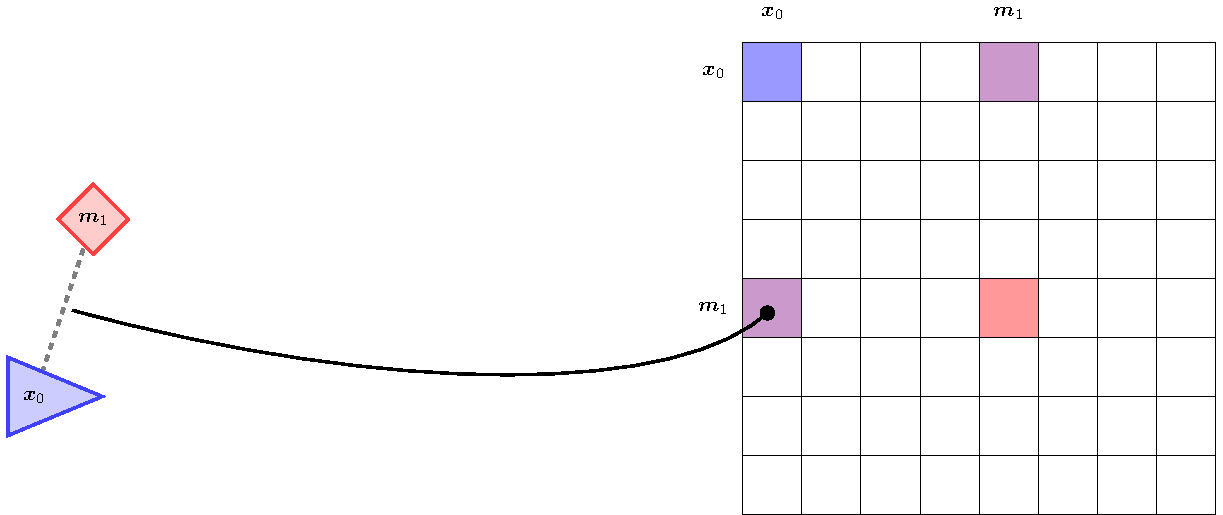
\includegraphics[width=\figScale\textwidth]{tikz/matrix1.pdf}
        \caption{Block addition to the information matrix $\bs{H}$ after a landmark measurement.}
        \label{fig:matrix1}
    \end{subfigure}
    \begin{subfigure}[htbp!]{\textwidth}
        \centering
        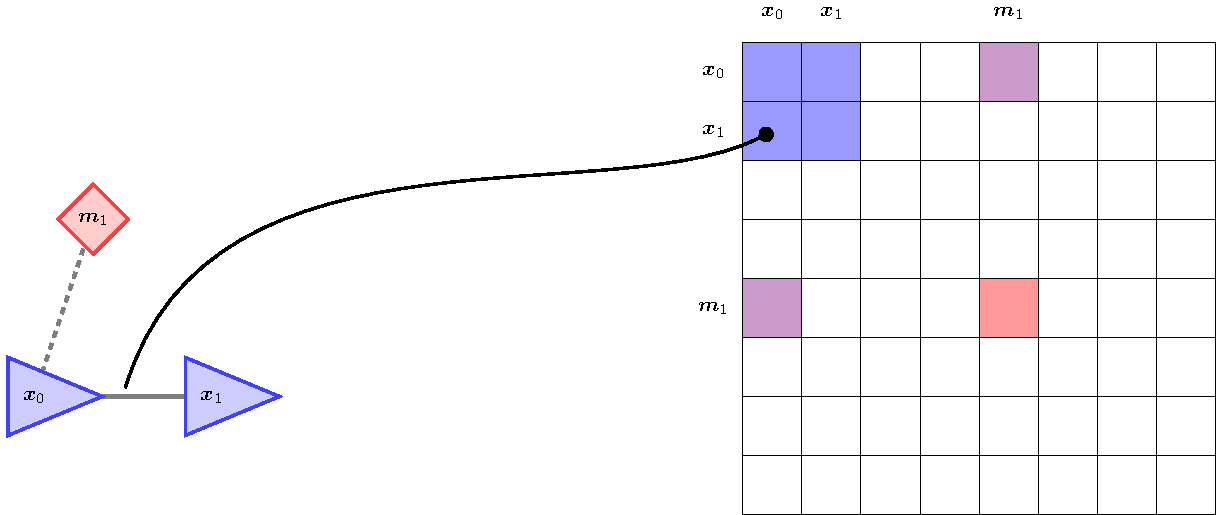
\includegraphics[width=\figScale\textwidth]{tikz/matrix2.pdf}
        \caption{Block addition to the information matrix $\bs{H}$ after a robot movement.}
        \label{fig:matrix2}
    \end{subfigure}
    \begin{subfigure}[htbp!]{\textwidth}
        \centering
        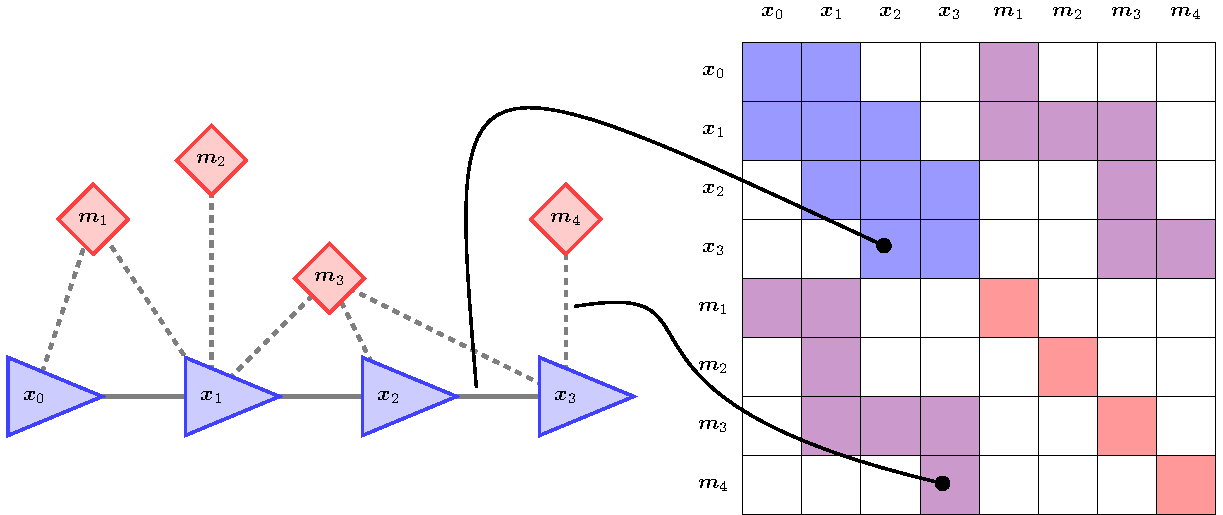
\includegraphics[width=\figScale\textwidth]{tikz/matrix3.pdf}
        \caption{Shows the block structure of the information matrix $\bs{H}$ after 3 robot movements and 7 measurements.}
        \label{fig:matrix3}
    \end{subfigure}
    \caption[Information matrix structure]{Progressing filling of the information matrix $\bs{H}$ as the robot moves and takes measurements. Blue: pose-pose block. Purple: pose-landmark block. Red: landmark-landmark block.}
    \label{fig:information-matrix}
\end{figure}

The information matrix can be divided in four submatrices. The top-left matrix (filled with blue squares) has the relative information between to pair of poses. Since the information acquired is only relative to two consecutive poses, 
this submatrix has a band diagonal structure, leaving all the other elements in zero. The top-right and bottom-left submatrices are equivalent, and contain the relative information between a pose and a measured landmark. The number of block in these matrices depends on the number of landmarks measured, but is often in SLAM that only spatially close landmarks are measured at every pose, leaving these matrices, again, with much of their elements in zero. Finally, the bottom-right submatrix regards information about pair of landmarks. Since there are not direct measurement between two landmarks, this submatrix is leaved as a block diagonal matrix.

Therefore it's shown that the number of non-zero elements in $\bs{H}$ is proportional to the number of edges in the graph, leading to a matrix with a large number of zero elements. This kind of matrices are called \it{sparse matrices}. Fast and efficient algorithm exist to solve~\eqref{eq:linear-system} for sparse matrices, such as Cholesky decomposition and Preconditioned Conjugate Gradient (PCG). These algorithms are already implemented in the g$^2$o framework that will be used.

\section{Review of the State of the Art in SLAM}
\label{sec:state-of-the-art}

SLAM as a probabilistic problem has its beginning in the 1986 IEEE Robotics and Automation Conference held in San Francisco, California~\cite{tutorial}. One of the first papers to give a solution to SLAM was \cite{ekfslam} using the Extended Kalman Filter technique. This solution is now known EKF SLAM.

One of the first papers to state SLAM as an optimization over a graph is~\cite{firstgraph} by Li and Milios. They were the first to treat motion and measurement in a equally as information constrains, which differed form standard EKF view where motion information is used for prediction, and measurement as correction for the Kalman filter.

The GraphSLAM algorithm as stated in this work was first presented in~\cite{graphslam} by Thrun and Montemerlo. In this paper the SLAM negative likelihood posterior is derived for solving the full SLAM problem, and the optimization problem is stated in a similar way as in section~\ref{sec:graphslam-description}. However, it not specify the way of solving the optimization in~\eqref{eq:minimization}. 

From there, several improvement have been made to the general idea of the GraphSLAM algorithm. In~\cite{sqrtsam} a similar graph representation is used to solve SLAM, called $\sqrt{\text{SAM}}$ (Square Root Smoothing and Mapping). In this context, \it{smoothing} corresponds to esimate the entire robot trajectory up to the current time. $\sqrt{\text{SAM}}$ uses the measurement Jacobian instead of the information matrix to represent the system uncertainty. Although they are equivalent in term of information, they have different computational properties. $\sqrt{\text{SAM}}$ can be used as a batch or an incremental algorithm for SLAM solving, and use either QR or Cholesky factorization of the linear equation solving, with variable ordering for complexity improvement. 

An updated version of $\sqrt{\text{SAM}}$, called iSAM, is presented in~\cite{isam}. It improves the performance in the incremental version, by directly updating the square root information matrix with new measurement as they arrive. It also avoids unnecessary fill-in in the information matrix generated by trajectory loop, by doing periodic variable reordering. It solves online data association using maximum likelihood and nearest neighbor matching.

Another improvement of iSAM is presented in~\cite{isam2}, iSAM2, in which they define a new data structure, called \it{Bayes Tree}, that allows them to improve the performance in the online case, by updating only the necessary variables in the linearization point after arrival of new data. 

In~\cite{robustloop} a robust consistency-based loop-closure verification method, Realizing Reversing and Recovering (RRR) algorithm, is presented for de detection and correction of incorrect loop closure generated by the SLAM algorithm. Incorrect loop closure appear when a robot visit similar looking locations, and can severely corrupt the map estimate.     

For efficiently solving graph optimization problems that appear in SLAM and other situations, a framework called g$^2$o (general graph optimization) is presented in~\cite{g2o}. g$^2$o is an open source optimization tool written in \verb!C++!.  It was designed to be easily extensible to a wide range of problems, and it contains typical optimization techniques used for sparse matrices, such as Cholesky decomposition and Preconditioned Conjugate Gradient. 

%The contribution of this work is to provide a fully functional GraphSLAM algorithm, which could be used for the navigation of robots in real world scenarios, and for the realization of comparative analysis with other SLAM algorithms.

\chapter{Methodology and Implementation}
\label{chap:implementation}
 
In this chapter the implementation of the GraphSLAM algorithm is presented and explained. The algorithm is capable of solving the SLAM problem in an offline manner for a 2D scenario, in the cases of known and unknown data association.

The g$^2$o framework used in this work provides of a least squares solver for the optimization of equation~\eqref{eq:minimization}, as well as a protocol to define the graph of the SLAM problem. g$^2$o is well optimized and it has several options for the solver, so the known correspondence version of the GraphSLAM algorithm is relative straightforward to implement.

However, g$^2$o doesn't provide a way to handle unknown data association, so the main goal of this work is to implement a method for solving the correspondence problem in an efficient manner.

\section{The g$^2$o Protocol}

The first step to implementing the GraphSLAM algorithm is to define a protocol to store and interpret the data on a graph. g$^2$o already provides such protocol. The stored data are of two types: data from nodes, and data from edges. 

In the SLAM context, nodes itself can be of two types, pose nodes and landmark nodes. Pose nodes represent the pose of the robot, in the 2D case they consist in 3 variables: robot's $x$ and $y$ position, and robot's orientation $\theta$. In g$^2$o a pose node is denoted with the keyword \texttt{VERTEX\_SE2}\footnote{Vertex is synonymous of node. SE2 is the Non-Euclidean space that consists of two spatial dimensions and a angular dimension.}. Landmark nodes represent the 2D position ($x$ and $y$) of a landmark. They are denoted with the keyword \texttt{VERTEX\_XY}.

Edges represents either robot's odometry (data of robot's change in position), or robot's measurements of landmarks. Odometry is measured as the difference between robot's pose at two consecutive timesteps: $(\Delta x, \Delta y, \Delta \theta)$. On the other hand, robot measurement are given as the $x$ and $y$ distance to the landmark relative to the robot reference frame. Figure~\ref{fig:protocol} illustrates the odometry an measurement of a robot. Keywords \texttt{EDGE\_SE2} and \texttt{EDGE\_SE2\_XY} are use to denote odometry and measurement edges respectively.

\begin{figure}[htbp!]
    \centering
    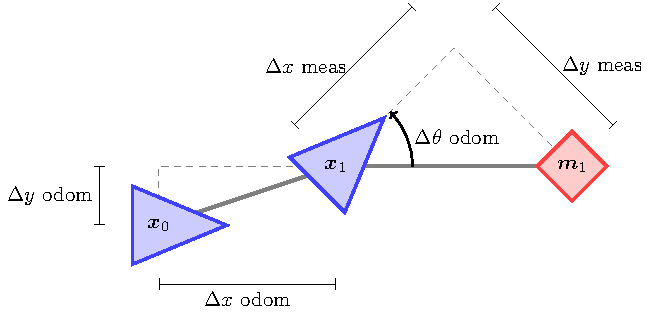
\includegraphics[width=0.7\textwidth]{tikz/protocol.pdf}
    \caption{Illustration of odometry and measurements values in g$^2$o.}
    \label{fig:protocol}
\end{figure}

For GraphSLAM to work correctly, one must also provide to the algorithm of the uncertainty of odometry and measurements. These correspond to the covariance matrices $\bs{R}_k$ and $\bs{Q}_k$ from motion~\eqref{eq:motion-model} and measurement~\eqref{eq:measurement-model} model respectively. g$^2$o works with the inverse of the covariance matrix, known as the information matrix. Nevertheless these representation are equivalent in terms of the knowledge of the system. Since covariance matrices (and their inverse) are symmetric, only the upper diagonal elements are needed. In this work it is assumed that the model uncertainties are time independent, i.e., all nodes have the same values for the information matrix. The notation of each element of the matrices is given by:

\begin{equation}
    \bs{R}^{-1}_k = \begin{pmatrix}
    ipxx & ipxy & ipxt\\
    ipxy & ipyy & ipyt\\
    ipxt & ipyt & iptt
    \end{pmatrix} \;\;
    \bs{Q}^{-1}_k = \begin{pmatrix}
    ilxx & ilxy\\
    ilxy & ilyy
    \end{pmatrix} 
    \label{eq:info-matrices}
\end{equation}

Finally, nodes must be indexed so they can be distinguishable form one another. This is indicated by an integer \texttt{id}. Ids are used in edges to indicate which two nodes the edge is connecting.

Table~\ref{tab:protocol} summarize the g$^2$o notation to represent nodes and edges.

\begin{table}[htbp!]
    \centering
    \begin{tabular}{|c|c|}
        \hline
        Graph element & Notation\\
        \hline
        Pose node & \texttt{VERTEX\_SE2 id x y t}\\
        Landmark node & \texttt{VERTEX\_SE2\_XY id x y}\\
        Odometry edge & \texttt{EDGE\_SE2 id1 id2 dx dy dt ipxx ipxy ipxt ipyy ipyt ipyy}\\
        Measurement edge & \texttt{EDGE\_SE2\_XY id1 id2 dx dy ilxx ilxy ilyy}\\
        \hline
    \end{tabular}
    \caption{g$^2$o protocol for node and edge definition.}
    \label{tab:protocol}
\end{table}

In this work, it is assumed that the first pose is known with absolute certainty, and is fixed to $(0,0,0)$. In g$^2$o, this is done by the command \texttt{FIX id}, where the id of the first pose is used. To use the data in the framework, it can be written in a plain text, which is then uploaded to g$^2$o.

The next code present a simple example of the g$^2$o protocol, its graphical equivalence is shown in Figure~\ref{fig:protocol-example}. In practice, when solving SLAM, only odometry and measurements are known, then only edges must be specified in the file:
 
\begin{lstlisting}[caption = g$^2$o protocol example, captionpos=b, basicstyle=\small]
VERTEX_SE2 0 0 0    0
FIX 0
VERTEX_SE2 1 4 0    0
VERTEX_SE2 2 4 4 1.57
VERTEX_SE2 3 0 4 3.14

VERTEX_XY 11 2 2
VERTEX_XY 12 6 2
VERTEX_XY 13 2 6

EDGE_SE2 0 1 4 0 1.57 1 0 0 1 0 1
EDGE_SE2 1 2 4 0 1.57 1 0 0 1 0 1
EDGE_SE2 2 3 4 0    0 1 0 0 1 0 1

EDGE_SE2_XY 0 11  2  2 1 0 1
EDGE_SE2_XY 1 11  2  2 1 0 1
EDGE_SE2_XY 1 12  2 -2 1 0 1
EDGE_SE2_XY 2 11  2  2 1 0 1
EDGE_SE2_XY 2 12 -2  2 1 0 1
EDGE_SE2_XY 2 13  2 -2 1 0 1
EDGE_SE2_XY 3 11 -2  2 1 0 1
EDGE_SE2_XY 3 13 -2 -2 1 0 1
\end{lstlisting}

\begin{figure}[htbp!]
    \centering
    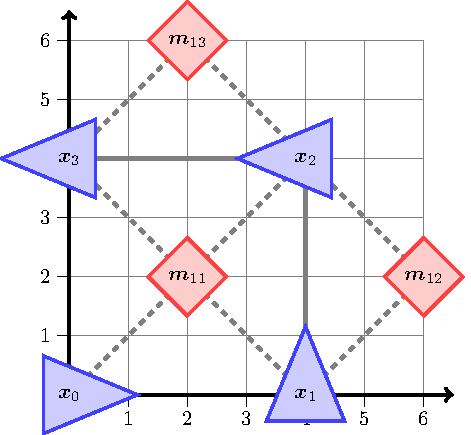
\includegraphics[width=0.5\textwidth]{tikz/protocol-example.pdf}
    \caption{Graphical representation of g$^2$o protocol example.}
    \label{fig:protocol-example}
\end{figure}

\section{The Known Correspondence Case}
\label{sec:known-asso-imp}

In the known correspondence case each measurement incorporates the information of the landmark sensed form the map. It is equivalent to know the correct values of \texttt{id1} and \texttt{id2} for every \texttt{EDGE\_SE2\_XY}. In a real world scenario, data association is usually not known, however, the known correspondence case is still useful in simulations to check the correctness of the algorithm.

With g$^2$o, solving the known correspondence case is just a matter of loading the data to the framework, set the desired parameters, and running the solver. 

The parameters that can be set in the solver includes: 

\begin{enumerate}
    \item The sparse solver for the inversion in~\eqref{eq:linear-system}: Cholesky solver, PCG solver
    \item The optimization algorithm for solving~\eqref{eq:linearized}-\eqref{eq:update}: Gauss-Newton, Levenberg-Marquardt
    \item The number of iteration for the algorithm to stop.
\end{enumerate}

For the sparse solver, g$^2$o uses third-parties libraries from which the user can choose: CHOLMOD, CSparse\footnote{CHOLMOD and CSparse can be found in \url{http://faculty.cse.tamu.edu/davis/suitesparse.html}}, Eigen\footnote{\url{http://eigen.tuxfamily.org/index.php?title=Main_Page}}. 

This work provides of a Python script to easily set the parameters of the framework and run the solver. It also provides of a 2D simulator that generates a robot path, landmarks and measurements. It's a modified version of the g$^2$o simulator that allows the user to set the information parameters from matrices~\eqref{eq:info-matrices} in the simulations. This make possible to test the GraphSLAM algorithm for different noise levels. The simulation also allows to compare the results with the \it{ground truth}. The ground is the true estimate to be achieved, and it's given by the simulator. 

The Python script is also able to generate an initial guess of the estimate using robot odometry and the first measurement of each landmark. The initial guess is used as a starting point for the optimization algorithm. Figure~\ref{fig:simulation} shows an example of the ground truth and the initial guess of a SLAM simulation.

\begin{figure}[htbp!]
    \centering
    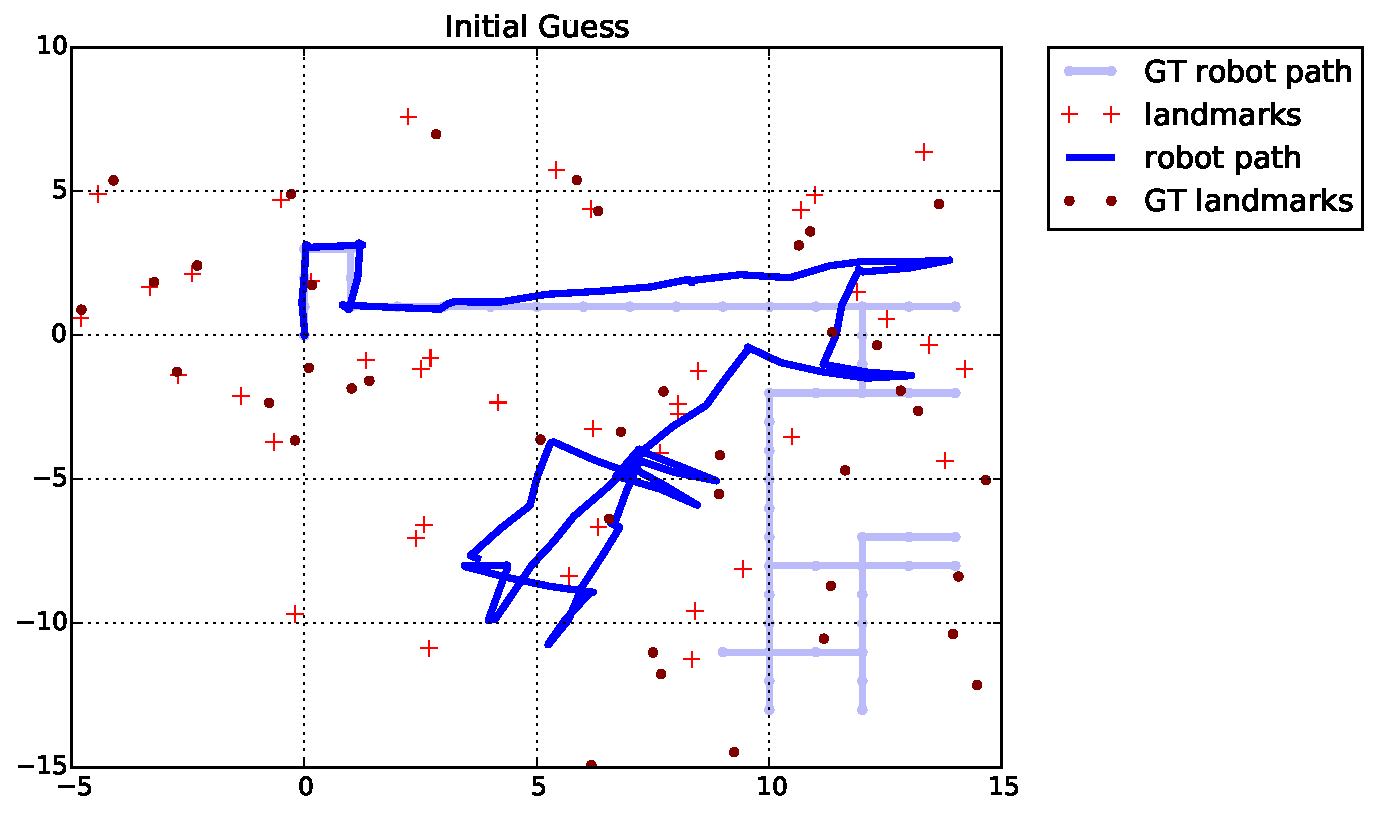
\includegraphics[width=0.8\textwidth]{imagenes/guess_op_100_oa_100_lp_100_ds_100.pdf}
    \caption[Example of an initialization of a SLAM simulation.]{Example of an initialization of a SLAM simulation. The light blue line is ground truth path, and dark red circles are ground truth landmark. The blue line is odometry path, and red crosses are the initial guess for landmarks.}
    \label{fig:simulation}
\end{figure}

The pseudocode for the known correspondence case is shown in Algorithm~\ref{alg:known-correspondence}.

\begin{algorithm}[htbp!]
    \caption{GraphSLAM Known Correspondence}
    \label{alg:known-correspondence}
    \begin{algorithmic}[1]
        \Require optimizer, data
        \State optimizer.setParameters(parameters)
        \State optimizer.loadData(data)
        \State optimizer.genInitialGuess()
        \State optimizer.solve(numberIterations)
        \State optimizer.writeData()
    \end{algorithmic}
\end{algorithm}

Optionally g$^2$o can use robust kernels to deal with \it{outliers}. An outlier is a corrupt measurement that doesn't follows the distribution assumed for the model. They are usually generated by sensors malfunctions and tend to have extreme values, far away form the expected measurement. 

From equation~\eqref{eq:simplified}, it can be seen that each error function has a quadratic influence in function $F(\bs{y})$. This means that a single outlier can significantly degrade the construction of $F$, and thus the result of the estimation. To mitigate this problem a robust kernel function can be applied to each error term $\bs{e}_{ij}(\bs{y})$ in~\eqref{eq:simplified}, so that high values of $\bs{e}_{ij}$ has reduced effect in $F$. Robust kernels included in g$^2$o are: Cauchy, DCS, Fair, GemanMcClure, Huber, PseudoHuber, Saturated, Tukey, Welsch. Most robust kernels must also specify the kernel's width, that is the point on the function in which the kernel effect start. Figure~\ref{fig:kernels} shows the plots of different kernels in g$^2$o. 

\begin{figure}[htbp!]
    \centering
    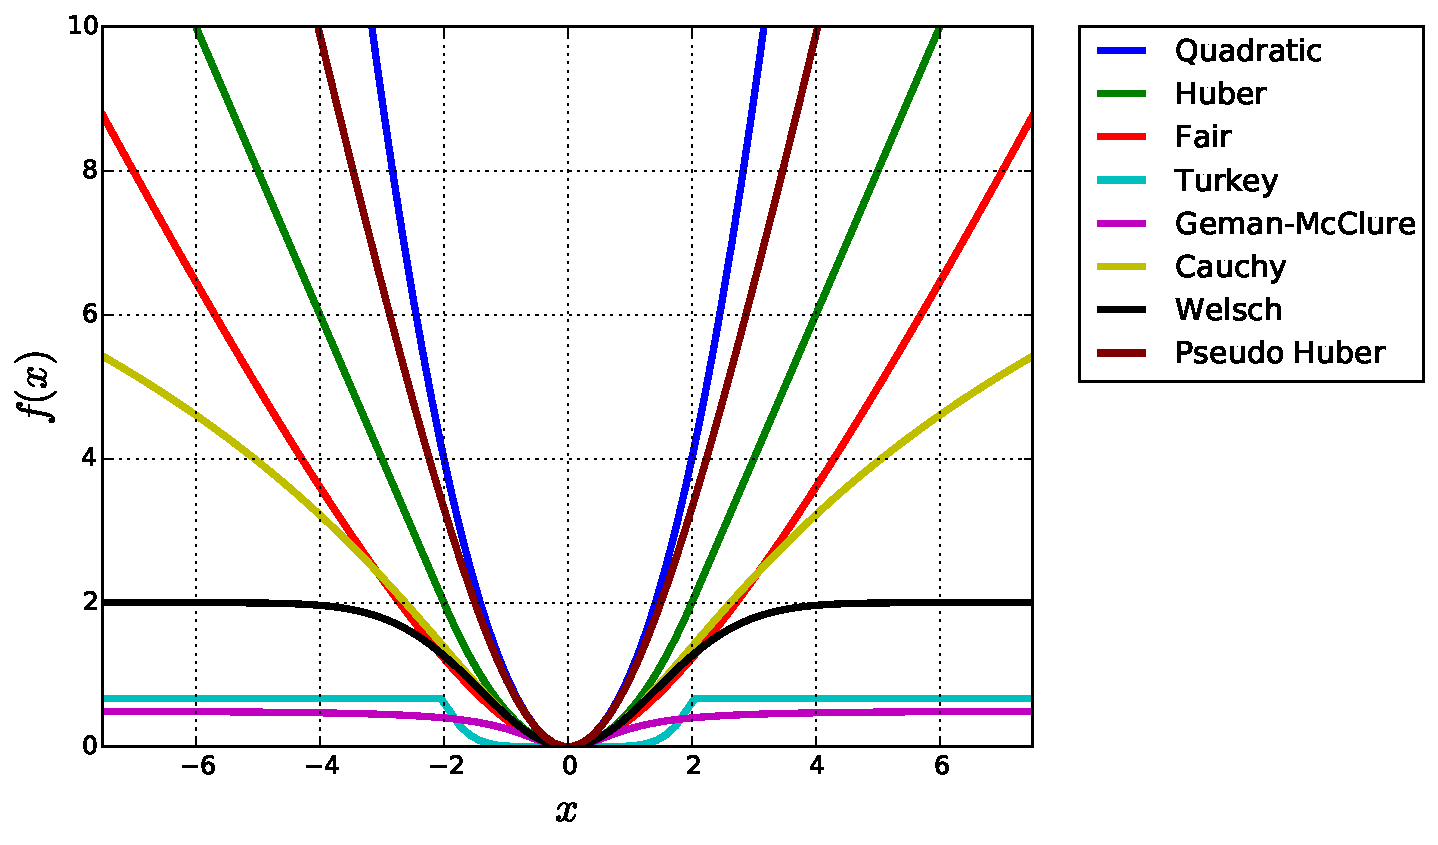
\includegraphics[width=0.8\textwidth]{imagenes/kernels.pdf}
    \caption[Plots of different kernels.]{Plots of different robust kernels with equals width, compared with the quadratic function.}
    \label{fig:kernels}
\end{figure}

\section{The Unknown Correspondence Case}

In the unknown correspondence case there is no information of which landmark generates each measurement, neither of how many landmarks are in the map. The g$^2$o framework does not provides a way to solve the correspondence problem, so a method must be developed to address the issue. In this work the method implemented is based in the one presented in~\cite{graphslam}, with some differences to take in account the speed of the algorithm. 

\subsection{The Correspondence Test}

The premise of the method is as follows: a correspondence test is developed to check the likelihood of two landmarks being the same. If the likelihood is high enough, the landmarks are merged into one. 

To justify mathematically this test, the variable $\bs{m}_{i,j}=(\bs{m}_i~ \bs{m}_j)^T$ is defined as de concatenation of landmarks $i$ and $j$. The posterior probability of $\bs{m}_{i,j}$ over the measurements and control inputs is given by:

\begin{equation}
p(\bs{m}_{i,j}|\bs{z}_{1:k},\bs{u}_{1:k})=
\det(2\pi\bs{\Sigma}_{\bs{m}_{i,j}})^{-\frac{1}{2}}\exp\left\lbrace -\frac{1}{2}(\bs{m}_{i,j}-\bs{\mu}_{\bs{m}_{i,j}})^T
\bs{\Sigma}_{\bs{m}_{i,j}}^{-1}(\bs{m}_{i,j}-\bs{\mu}_{\bs{m}_{i,j}})\right\rbrace
\label{eq:concatenate}
\end{equation}

Where $\bs{\mu}_{\bs{m}_{i,j}}=(\bs{\mu}_{\bs{m}_i}~ \bs{\mu}_{\bs{m}_j})^T$ is the current estimate of the landmarks $i$ and $j$. Matrix $\bs{\Sigma}_{\bs{m}_{i,j}}$ is the covariance matrix marginalized over landmarks $i$ and $j$. Since it has been assumed a normal distribution for the estimate, this covariance can be computed using the marginalization lemma~\cite{graphslam}. In practice, g$^2$o provides a function to compute $\bs{\Sigma}_{\bs{m}_{i,j}}$.

Then, to compare $\bs{m}_i$ and $\bs{m}_j$ another variable is defined as the difference between the two landmarks: $\bs{\Delta}_{i,j}=\bs{m}_i-\bs{m}_j$, or alternatively, using the difference matrix:

\begin{align}
D &= \begin{pmatrix}
1 & 0\\
0 & 1\\
-1 & 0\\
0 & -1
\end{pmatrix}\\
\Rightarrow 
\bs{\Delta}_{i,j}&=\bs{m}_i-\bs{m}_j = D^T\bs{m}_{i,j}
\end{align}

It can be proven that $\bs{\Delta}_{i,j}$ is distributed as $\Nn(D^T\bs{\mu}_{\bs{m}_{i,j}}, D^T \bs{\Sigma}_{\bs{m}_{i,j}} D)\defi \Nn(\bs{\mu}_{\bs{\Delta}_{i,j}}, \bs{\Sigma}_{\bs{\Delta}_{i,j}})$. Then its PDF is given by:

%To justify mathematically this test, the variable $\bs{\Delta}_{i,j}=\bs{m}_i-\bs{m}_j$ is defined as the difference in position of landmark $\bs{m}_i$ and $\bs{m}_j$. The posterior probability of $\bs{\Delta}_{i,j}$ over the measurements and control inputs is given by:

\begin{equation}
p(\bs{\Delta}_{i,j}|\bs{z}_{1:k},\bs{u}_{1:k})=
\det(2\pi \bs{\Sigma}_{\bs{\Delta}_{i,j}})^{-\frac{1}{2}}\exp\left\lbrace -\frac{1}{2}(\bs{\Delta}_{i,j}-\bs{\mu}_{\bs{\Delta}_{i,j}})^T
\bs{\Sigma}_{\bs{\Delta}_{i,j}}^{-1}(\bs{\Delta}_{i,j}-\bs{\mu}_{\bs{\Delta}_{i,j}})\right\rbrace
\label{eq:correspondence-test}
\end{equation}

%Where $\bs{\mu}_{\bs{\Delta}_{i,j}}$ is the current estimate of the landmark's difference. It can be easily computed as $\bs{\mu}_{\bs{m}_i}-\bs{\mu}_{\bs{m}_j}$, where $\bs{\mu}_{\bs{m}_i}$ and $\bs{\mu}_{\bs{m}_j}$ are the current estimate of both landmarks.

%Matrix $\bs{\Sigma}_{\bs{\Delta}_{i,j}}$ is the covariance matrix marginalized over landmarks $i$ and $j$. Since it has been assumed a normal distribution for the estimate, $\bs{\Sigma}_{\bs{\Delta}_{i,j}}$ can be computed using the marginalization lemma~\cite{graphslam}. In practice, g$^2$o provides a function to compute $\bs{\Sigma}_{\bs{\Delta}_{i,j}}$.

When two landmarks are equivalent it is expected that their position is the same, hence $\bs{\Delta}_{i,j}=0$. Evaluating this in the posterior probability~\eqref{eq:correspondence-test} gives the likelihood of landmark equivalence:

\begin{equation}
\pi_{j=k} \defi
p(\bs{\Delta}_{i,j}=0|\bs{z}_{1:k},\bs{u}_{1:k})=
\det(2\pi\bs{\Sigma}_{\bs{\Delta}_{i,j}})^{-\frac{1}{2}}
\exp\left\lbrace-\frac{1}{2}\bs{\mu}_{\bs{\Delta}_{i,j}}^T\bs{\Sigma}_{\bs{\Delta}_{i,j}}^{-1}\bs{\mu}_{\bs{\Delta}_{i,j}}\right\rbrace
\label{eq:landmark-equivalence}
\end{equation}

The correspondence test consist in assert a landmark equivalence when the likelihood $\pi_{j=k}$ is greater that a user defined threshold $\chi$. Intuitively a greater threshold means being more strict in considering a landmark merging.

\subsection{The Unknown Correspondence Algorithm}

Once the correspondence test is defined, it can be used to implement an GraphSLAM algorithm with unknown data association. 

The algorithm works as follows: first all landmarks are initialized as if each measurement correspond to an individual landmark. The correspondence test is run over every possible pair of landmarks, merging landmarks that pass the test. After the tests are finished, the estimate is updated running the solver in the same way as in the case of known correspondence. After the solver, the correspondence tests are run again, and the solver is run afterward. Correspondence test and solver are alternated until no new landmark associations are found. 

Algorithm~\ref{alg:unknown-correspondence} presents the unknown correspondence algorithm in pseudocode. 

\begin{algorithm}[htbp!]
    \caption{GraphSLAM Unknown Correspondence}
    \label{alg:unknown-correspondence}
    \begin{algorithmic}[1]
        \Require optimizer, data
        \State optimizer.setParameters(parameters)
        \State optimizer.loadData(data)
        \State optimizer.genInitialGuess()
        \State
        \While{association found} 
            \ForAll{pair of landmark ($i$,$j$)} 
                \If{correspondenceTest($i$,$j$) $\geq \chi$} 
                    \State optimizer.merge($i$,$j$) 
                \EndIf 
            \EndFor
            \State optimizer.solve(numberIterations)
        \EndWhile
        \State
        \State optimizer.writeData()
    \end{algorithmic}
\end{algorithm}

\subsection{Speeding up the Unknown Correspondence Algorithm}

Algorithm~\ref{alg:unknown-correspondence} is inefficient. In particular the correspondence test is run over every pair of landmarks at each iteration. The number pairs is quadratic in the number of landmarks, furthermore, even landmarks that are obviously not equivalent, such as landmarks greatly separated, are tested. Empirical testing have shown that the bottleneck of the algorithm is the correspondence test, in particular, the computation of the marginalized covariance $\bs{\Sigma}_{\bs{\Delta}_{i,j}}$, so is necessary call this function as less often as possible. The optimization of the algorithm is essential to run GraphSLAM in large datasets. The next subsections presents the strategies adopted to improve the algorithm performance.

\subsubsection{Incremental Optimization}

Incremental optimization is based in the following principle: landmarks measured late in the robot's path are subject to the accumulated error of all past robot's poses. This fact is can be visualized in the simulation in Figure~\ref{fig:simulation}. Due to this, equivalent landmarks found late in the trajectory will be merged only when all the previous estimates of the pose has already been corrected by the algorithm. Testing correspondence between these landmarks earlier is pointless, simply because their error is to high to produce an association. 

A way to deal with this problem is to test association only for landmarks measured in early poses, and then test for late poses when the path is corrected. An extreme version of this is the \emph{incremental optimization} algorithm: at each iteration consider only the current pose. Test landmarks observed in current pose with landmarks from all previous poses, and then run the solver. In the next iteration do the same for the next pose, and repeat until the last pose. Intuitively, the algorithm is incrementally correcting the path with early measured landmarks, which have low uncertainty, until all path is corrected. Figure~\ref{fig:incremental} illustrate the working of the incremental optimization for a simple example.

\begin{figure}[htbp!]
    \centering
    \begin{subfigure}[htbp!]{0.25\textwidth} 
    \centering
    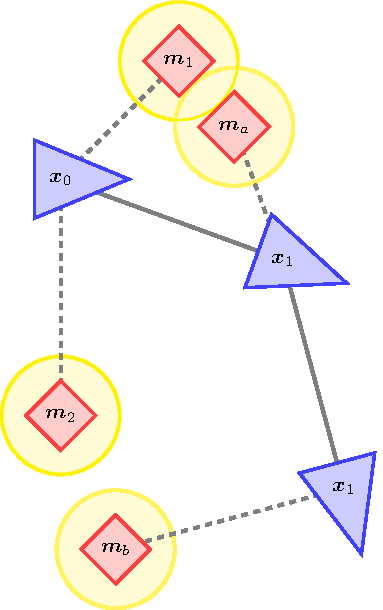
\includegraphics[width=\textwidth]{tikz/incremental1.pdf}
    \caption{Initial guess.}
    \end{subfigure}\hspace{2em}
    \begin{subfigure}[htbp!]{0.25\textwidth} 
        \centering
        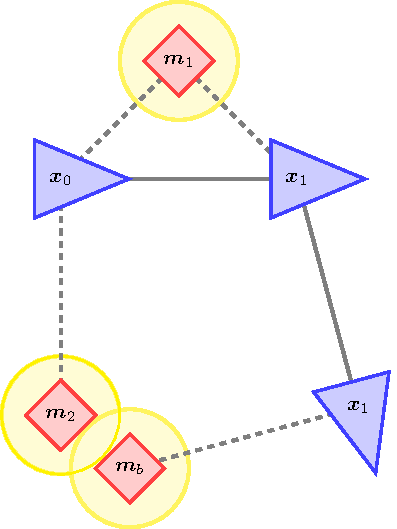
\includegraphics[width=\textwidth]{tikz/incremental2.pdf}
        \caption{Estimate after associating $m_1$ and $m_a$, and running the solver.}
    \end{subfigure}\hspace{2em}
    \begin{subfigure}[htbp!]{0.25\textwidth} 
        \centering
        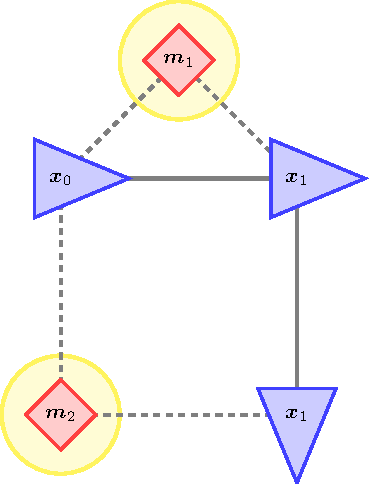
\includegraphics[width=\textwidth]{tikz/incremental3.pdf}
        \caption{Estimate after associating $m_2$ and $m_b$, and running the solver.}
    \end{subfigure}
    \caption[Example of the incremental optimization.]{Example of the incremental optimization. The yellow circle represents the landmark uncertainty. Note that at first is not possible to associate landmarks $\bs{m}_2$ and $\bs{m}_b$ because $\bs{m}_b$ has the accumulated error of $\bs{x}_1$ and $\bs{x}_2$. It's not until the association between $\bs{m}_1$ and $\bs{m}_a$, observed in previous poses, is made that the latter landmarks can be merged.}
    \label{fig:incremental}
\end{figure}    
The incremental optimization has a subtle flaw, once a correspondence test is run between two landmark, it's never tested again, since only current measurements are tested. If a test failed at some point, but posterior correction make it possible for the test to pass, this association will be miss. It is expected that this situation doesn't occur often, since the incremental optimization algorithm usually gives a good estimate of the path up to the current pose. Nevertheless, this error is absolutely possible.

To mitigate this problem, \emph{full optimizations} can be run occasionally along with the incremental optimization. Full optimization consists in testing correspondence between all possible pair of measured landmarks up to the current pose, in a similar fashion as it is done in Algorithm~\ref{alg:unknown-correspondence}. This way a compromise can be achieved between the algorithm speed and performance. In this implementation the user is able to choose the frequency with which the full optimization are run It is done by setting the parameter $io$ (inter full optimizations), which is the number of incremental optimization performed between two full optimizations. 

\subsubsection{Pose Skipping}

The incremental optimization algorithm described above run the solver and produce an optimization every time after a new pose is analyzed. In some cases the solver optimization becomes the bottleneck rather than the data association. In these cases it is convenient to  test association between several consecutive poses after running the solver.

this strategy is named \it{pose skipping}, where a parameter $ps$ is introduced to control the number poses to be skipped after the next optimization. If $ps=n$ it indicated that the next optimization will be executed $n$ poses after the current pose. By default $ps=0$ (no skipping is made).    

\subsubsection{Distance Test}

Even with incremental optimization, there are still a lot of landmarks that are unnecessarily tested. The distance test strategy attempts to avoid testing landmarks that are widely separated, and thus are obviously not equivalent. To do this, a distance threshold is defined, with which, every pair of landmarks separated by a greater distance automatically fail the test. 

Defining a value for the threshold is non trivial. Two method are implemented. The first one is by user defined input. If the user has prior knowledge of the robot or the map, he/she could make a good estimate of the maximum distance between measurements from the same landmark. Then the user can set the distance threshold to this value.

Even if the maximum distance is not known a priori, a threshold value can still be calculated. Consider the threshold $\chi$ for the correspondence test in Algorithm~\ref{alg:unknown-correspondence}, for a given value of $\chi$, there exist a distance for which, even in the best case scenario, landmarks separated by this distance or more with never be associated. To prove this, consider the random variable for the distance  $\bs{\delta}_{i,j}$ between two landmarks. Its PDF is given by:

\begin{align}
p(\bs{\delta}_{i,j}|\bs{z}_{1:k},\bs{u}_{1:k})&=
\frac{1}{\sqrt{2\pi\sigma_{\bs{\delta}_{i,j}}^2}}
\exp\left\lbrace -\frac{(\bs{\delta}_{i,j}-\bs{\mu}_{\bs{\delta}_{i,j}})^2}{2\sigma_{\bs{\delta}_{i,j}}^2}\right\rbrace\\
d_{i=j} \defi p(\bs{\delta}_{i,j}=0|\bs{z}_{1:k},\bs{u}_{1:k})&=
\frac{1}{\sqrt{2\pi\sigma_{\bs{\delta}_{i,j}}^2}}
\exp\left\lbrace -\frac{\bs{\mu}_{\bs{\delta}_{i,j}}^2}{2\sigma_{\bs{\delta}_{i,j}}^2}\right\rbrace 
\end{align}

Which is equivalent to the PDF $p(\bs{\Delta}_{i,j}|\bs{z}_{1:k},\bs{u}_{1:k})$ in \eqref{eq:correspondence-test}, for the one dimensional case. $\bs{\mu}_{\bs{\delta}_{i,j}}^2$ is the euclidean distance between the mean of the landmarks, and $\sigma_{\bs{\delta}_{i,j}}^2$ is the variance of $p(\bs{\Delta}_{i,j}|\bs{z}_{1:k},\bs{u}_{1:k})$ projected in the line between $\bs{\mu}_{\bs{\Delta}_{i,j}}^2$ and $(0,0)$. For this analysis, the exact value of $\sigma_{\bs{\delta}_{i,j}}^2$ is not important.

The maximum distance at which association can still be made is given by the following problem:

\begin{equation}
\underset{d_{i=j}\geq\chi}{\text{max}}~~  |\bs{\mu}_{\bs{\delta}_{i,j}}|
\label{eq:max-distance}
\end{equation}

Considering only the positive values of $\bs{\mu}_{\bs{\delta}_{i,j}}$, $d_{i=j}$ becomes a decreasing function. By this fact, it can be seen that maximum at~\eqref{eq:max-distance} is achieved when $d_{i=j}=\chi$. A visual demonstration of this is shown in Figure~\ref{fig:max-distance}. Expanding the equality found:

\begin{align}
d_{i=j} &= \chi\\
\frac{1}{\sqrt{2\pi\sigma_{\bs{\delta}_{i,j}}^2}}
\exp\left\lbrace -\frac{\bs{\mu}_{\bs{\delta}_{i,j}}^2}{2\sigma_{\bs{\delta}_{i,j}}^2}\right\rbrace &= \chi \\
\exp\left\lbrace -\frac{\bs{\mu}_{\bs{\delta}_{i,j}}^2}{2\sigma_{\bs{\delta}_{i,j}}^2}\right\rbrace&= \sqrt{2\pi\sigma_{\bs{\delta}_{i,j}}^2} \chi\\
\bs{\mu}_{\bs{\delta}_{i,j}} &= \sqrt{-2\sigma_{\bs{\delta}_{i,j}}^2\log(\sqrt{2\pi\sigma_{\bs{\delta}_{i,j}}^2} \chi)} \label{eq:max-distance-exp}
\end{align}

So the maximum distance for an association is given by~\eqref{eq:max-distance-exp}. Unfortunately the distance is a function of $\sigma_{\bs{\delta}_{i,j}}^2$, which is computationally expensive to get. However expression~\eqref{eq:max-distance-exp} is concave in $\sigma_{\bs{\delta}_{i,j}}^2$, so a global maximum can be found (see Figure~\ref{fig:max-variance}). Intuitively this means that neither a large nor a low value of $\sigma_{\bs{\delta}_{i,j}}^2$ is good for associating landmarks at great distances. 

\begin{figure}[htbp!]
    \centering
    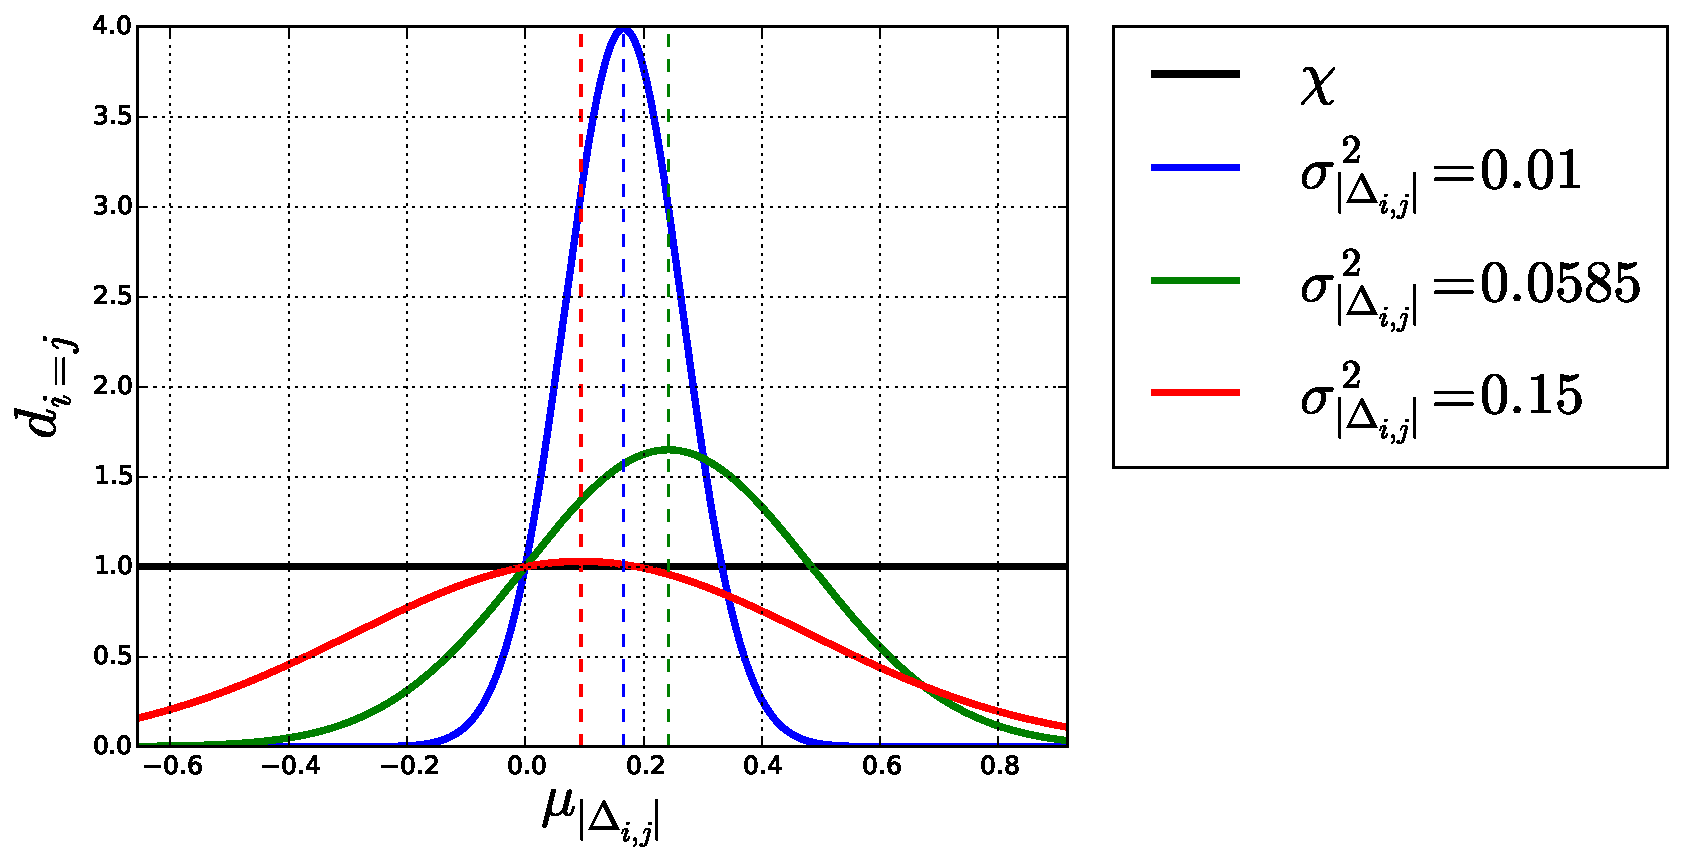
\includegraphics[width=0.7\textwidth]{imagenes/maxDistance.pdf}
    \caption[Plots of the PDF of the distance between two landmarks.]{Plots of the PDF of the distance between two landmarks for different values of $\sigma_{\bs{\delta}_{i,j}}^2$. The plots shows that maximum distance from zero is achieve when, $d_{j=k}=\chi$. Note that the function that achieve more distance is neither the one with more nor with less variance.}
    \label{fig:max-distance}
\end{figure}

\begin{figure}[htbp!]
    \centering
    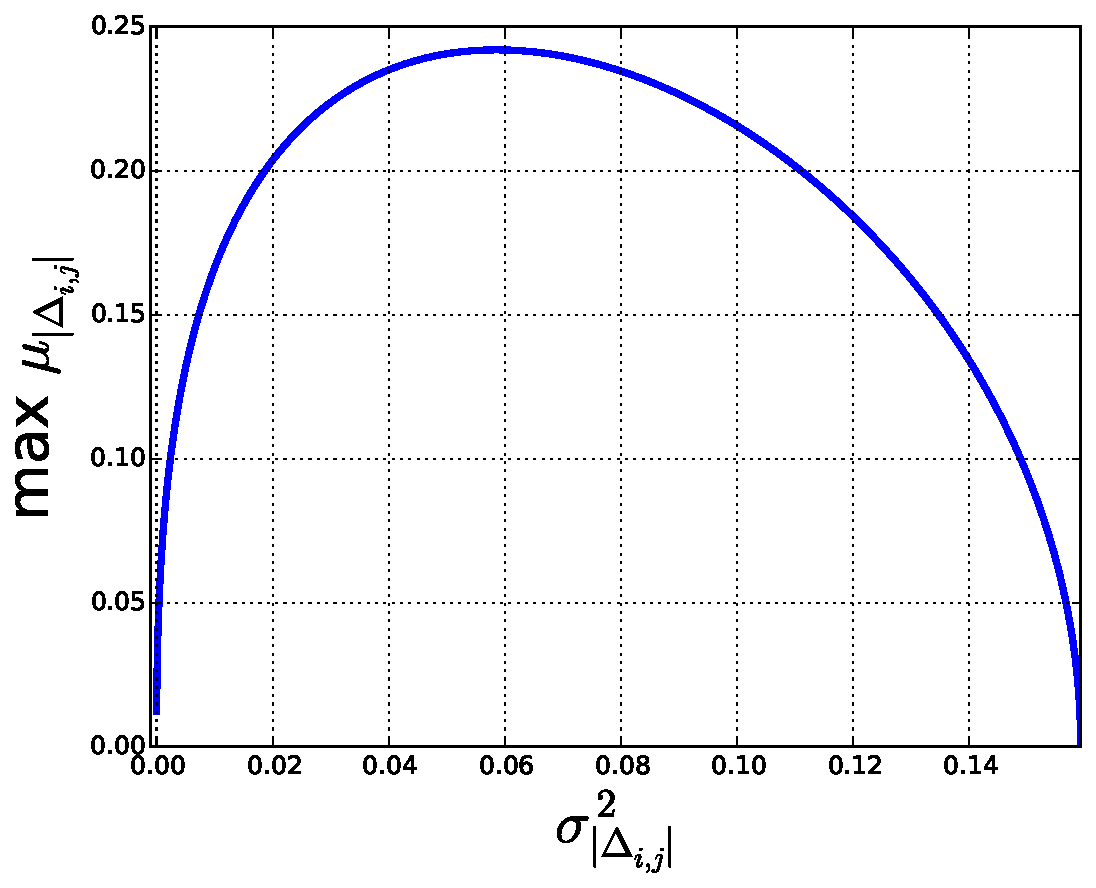
\includegraphics[width=0.5\textwidth]{imagenes/maxVariance.pdf}
    \caption[Plot of the maximum distance $\bs{\mu}_{\bs{\delta}_{i,j}}$ in function of $\sigma_{\bs{\delta}_{i,j}}^2$.]{Plot of the maximum distance $\bs{\mu}_{\bs{\delta}_{i,j}}$ in function of $\sigma_{\bs{\delta}_{i,j}}^2$. It can be seen that is a concave function.}
    \label{fig:max-variance}
\end{figure}

Using differential calculus it can be found maximum of $\bs{\mu}_{\bs{\delta}_{i,j}}$ for $\sigma_{\bs{\delta}_{i,j}}^2$ is achieved in $\sigma_{\bs{\delta}_{i,j}}^2 = \frac{1}{2\pi e\chi}$, which yields a value of $\bs{\mu}_{\bs{\delta}_{i,j}} = \frac{1}{\sqrt{2\pi e}\chi}$.  
This value can be used as a  distance threshold that only depends on $\chi$. The disadvantage of this method is that the threshold computed tend to be large relative to the problem, so the amount of correspondence tests avoided is limited.

\section{The Final Algorithm}

The final version of the implemented GraphSLAM algorithm solves the SLAM problem for unknown correspondence, it incorporates the incremental optimization, pose skipping and  distance test strategies to speed up the algorithm.

The algorithm of the final version of GraphSLAM is presented in Algorithm~\ref{alg:final}. $ps$ and $io$ correspond to the parameters for pose skipping and inter full optimization. To check if it is the right time to use either of the strategies, the module ($\%$) operator is used between the pose number and the parameter. 

\begin{algorithm}[htbp!]
    \caption{GraphSLAM Final Version}
    \label{alg:final}
    \begin{algorithmic}[1]
        \Require optimizer, data
        \State optimizer.setParameters(parameters)
        \State optimizer.loadData(data)
        \State optimizer.genInitialGuess()
        \State
        \ForAll{poses $p$}
        \State \Call{incrementalDataAssociation}{p}
        \If{$p~\%~ps = 0$}
        \State optimizer.solve(numberIterations)
        \EndIf
        \If {$p~\%~io = 0$}
        \State \Call {fullOptimization}{p}
        \EndIf
        \EndFor
        \State
        \State optimizer.writeData()
    \end{algorithmic}
\end{algorithm}

The GraphSLAM algorithm calls to functions, \texttt{intremental\-Data\-Association} and \texttt{full\-Optiomization}. The \texttt{intrementalDataAssociation} function tries to associate the landmarks observed in the current pose, with the previous landmarks. Its pseudocode is shown in Algorithm~\ref{alg:incremental-data-association}. The distance test is performed in line~\ref{line:distance-test}, where $dt$ is the maximum distance accepted for an association. \texttt{full\-Optimization} function search associations between all previous poses up to the current pose, and then run the solver. It can be done bt calling \texttt{intremental\-Data\-Association} iteratively, as shown in~\ref{alg:full-optimization}.

\begin{algorithm}[htbp!]
    \caption{Incremental Data Association Function}
    \label{alg:incremental-data-association}
    \begin{algorithmic}[1]
        \Function{incrementalDataAssociation}{$p$}
        \ForAll {landmarks $l_p$ observed in $p$}
        \ForAll {previous poses $q$ up to $p$}
        \ForAll {landmarks $l_q$ observed in $q$}
        \If {distance($l_p$,$l_q$) < $dt$} \label{line:distance-test}
        \If{correspondenceTest($i$,$j$) $\geq \chi$} 
        \State optimizer.merge($i$,$j$) 
        \EndIf
        \EndIf
        \EndFor
        \EndFor
        \EndFor
        \EndFunction
    \end{algorithmic}
\end{algorithm}

\begin{algorithm}[htbp!]
    \caption{Full Optimization Function}
    \label{alg:full-optimization}
    \begin{algorithmic}[1]
        \Function{fullOptimization}{$p$}
        \While{association found} 
        \ForAll {previous poses $q$ up to $p$} 
        \State \Call{IncrementalDataAssociation}{$q$}
        \EndFor
        \State optimizer.solve(numberIterations)
        \EndWhile
        \EndFunction
    \end{algorithmic}
\end{algorithm}

 
 

\chapter{Results}
\label{chap:results}

In this chapter the results of the GraphSLAM algorithm are presented for different test scenarios. In Section~\ref{sec:known-asso-res} the algorithm is tested for the simple case of known data association and simulated data. A parameters variation analysis is made, and their effect in the path estimation is shown. In Section~\ref{sec:unknown-asso-res} a similar analysis is performed, but for the case of unknown data association. In this case, new parameters related to the data association algorithm are tested. Finally in Section~\ref{sec:real-data-res}, the GraphSLAM algorithm is run in more realistic data. This data includes a robot simulated with Gazebo\footnote{http://gazebosim.org/}, a much more realistic robot simulator, and data obtained from real robots in outdoor environments. 

Through these tests several parameters and methods must be chosen for the algorithm to work properly. To limit the scope of this work, the sparse solver and the optimization algorithm are fixed and used in all the following tests. CSpase library and the Cholesky decomposition is used for the sparse solver, and the Levenberg-Marquardt method is used as the optimization algorithm. Also whenever the robust kernel method is used, Huber is the chosen kernel function (see Section~\ref{sec:known-asso-imp}). 

\section{Known Data Association}
\label{sec:known-asso-res}

The known data association case is the easiest one of the three scenarios, because correspondence between landmarks is given a priori. In this case Algorithm~\ref{alg:known-correspondence} is used. 

The parameters to be set in this case are the following:

\begin{itemize}
    \item $n_p$: number of poses of the robot path.
    \item $n_l$: number of landmarks in the map.
    \item $i_{op}$: odometry position information (inverse of variance).
    \item $i_{oa}$: odometry angle information.
    \item $i_{lp}$: landmark position information.
    \item $it$: number of iterations for the optimization algorithm to stop.
    \item $k_w$: Width of the chosen robust kernel.
\end{itemize}

Where $n_p$, $n_l$, $i_{op}$, $i_{oa}$, and $i_{lp}$ are parameters regarding the robot behavior in the test. They are passed to the simulator. The parameters $it$ and $k_w$ define de optimization strategy.

Through all the test made in this work, it is assumed that the information matrix of odometry and measurements models (same as~\eqref{eq:info-matrices}) are diagonal, i.e., their variables are not correlated. Furthermore, it is assumed that these matrices have the following structure:

\begin{equation}
\bs{R}^{-1}_k = \begin{pmatrix}
i_{op} & 0 & 0\\
0 & i_{op} & 0\\
0 & 0 & i_{oa}
\end{pmatrix} \;\;
\bs{Q}^{-1}_k = \begin{pmatrix}
i_{lp} & 0\\
0 & i_{lp}
\end{pmatrix} 
\label{eq:info-matrices-tests}
\end{equation}

This means that the robot experiences same uncertainty in the $x$ and $y$ axis, for both, motion and measurement model. 

\nameref{sec:test-i} is run with the parameters of Table~\ref{tab:test-i}. 

The simulation is constrained to a 2D world with $x\in[-15,15]$, $y\in[-15,15]$. At each step the simulator moves the robot 1 unit of distance and in turns randomly an angle of $\theta=0^\circ$, $90^\circ$, or $-90^\circ$. All simulations start from at $(0,0)$.

A kernel width of 1 unit is chosen heuristically, looking at the distance between landmarks. Intuitively, the user should set the kernel width to a distance in which two landmarks are unlikely to be the same, and therefore it corresponds to an outlier.

The results of the test are shown in Figure~\ref{fig:test-i}. In Figure~\ref{fig:test-ia} the initial guess is plotted on the left, and the posterior estimation after the solver on the right. The groundtruth is added in both graphs for comparison. Landmarks not observed by the robot are not shown.  It can be seen that the path of the initial guess rapidly diverges from the real solution. On the other hand, the solver estimation fits quite well with the groundtruth, both for the path and the landmarks.

To have a more quantitative view of the error made by the solver, the cumulative path error for every step is shown in Figure~\ref{fig:test-ib}.  The cumulative normalized error is given by:

\begin{equation}
error (i) = \frac{1}{i} \sum_{i} ||pos_{GT}-pos_{est}||
\end{equation} 

Where $i$ is the path's timestep. $pos_{GT}$ and $pos_{est}$ are the groundtruth and estimated position respectively. Then the error is the sum of the Euclidean distance of both positions, normalized by the number of steps. 

It can be seen that the error start increasing early in the path, but then it get stabilized. This is the effect of aggregating the information of the measurements and running the optimizer. As long as the robot keep measuring the same landmarks, it can maintain its error low. 


\afterpage{
\clearpage
\subsubsection{Test I.}
\label{sec:test-i}
\begin{table}[htbp!]
\centering
\begin{tabular}{|c|c|c|c|c|c|c|}
\hline
$n_p$ & $n_l$ & $i_{op}$ & $i_{oa}$ & $i_{lp}$ & $it$ & $k_w$\\
\hline \hline
300 & 40 & 1000 & 1000 & 1000 & 20 & 1\\
\hline 
\end{tabular}
\caption{Parameters for Test I.}
\label{tab:test-i}
\end{table}

\begin{figure}[htbp!]
\centering
\begin{subfigure}[b]{\estWidth\textwidth}
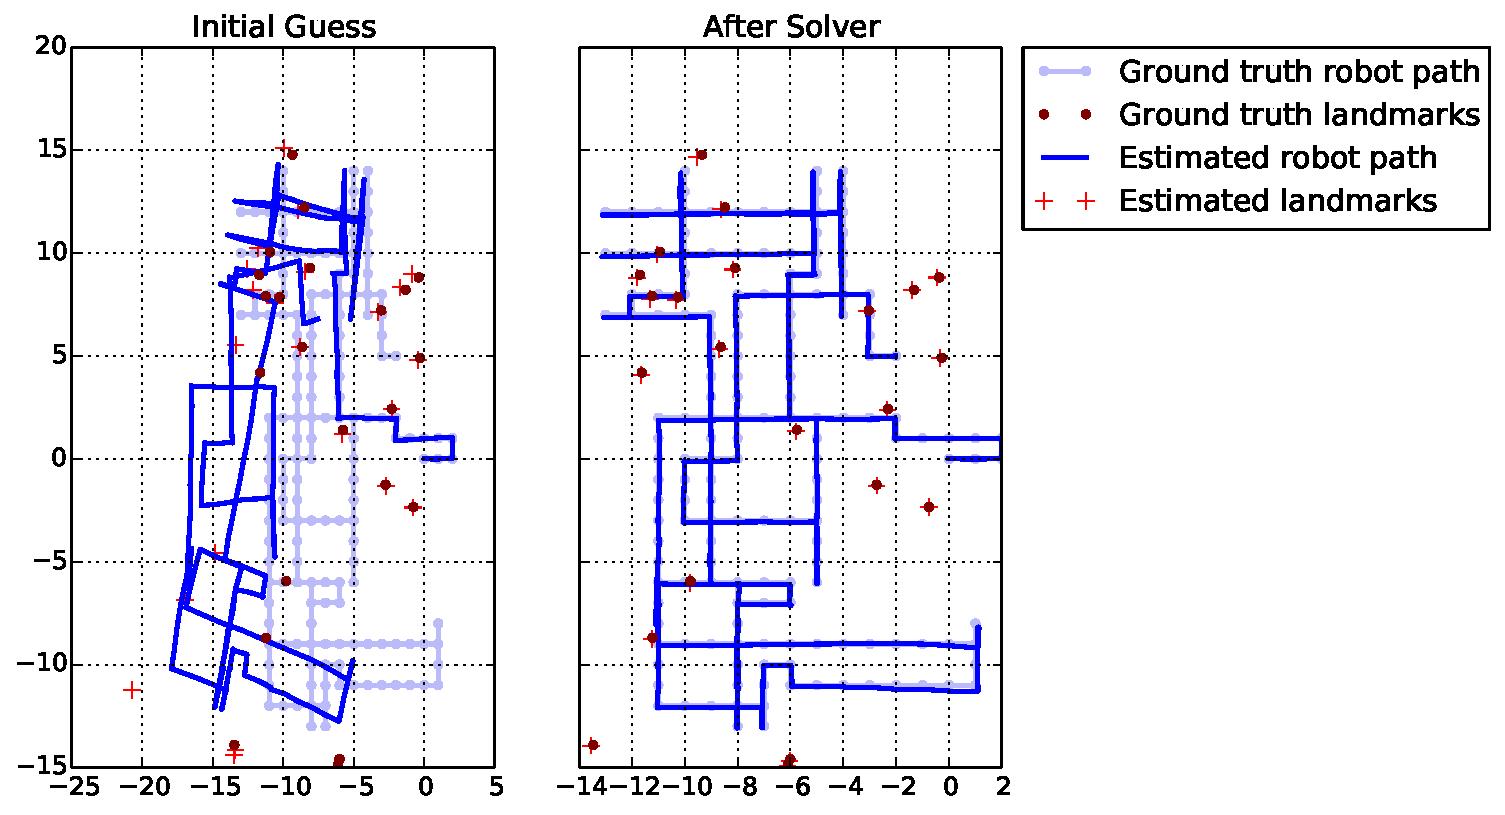
\includegraphics[width=\textwidth]{imagenes/tests/known/res_it_20_nl_40_op_1000_oa_1000_lp_1000_ds_300_kw_1.pdf}
\caption{Initial guess and solver estimation.}
\label{fig:test-ia}
\end{subfigure}\\
\begin{subfigure}[b]{\errorWidth\textwidth}
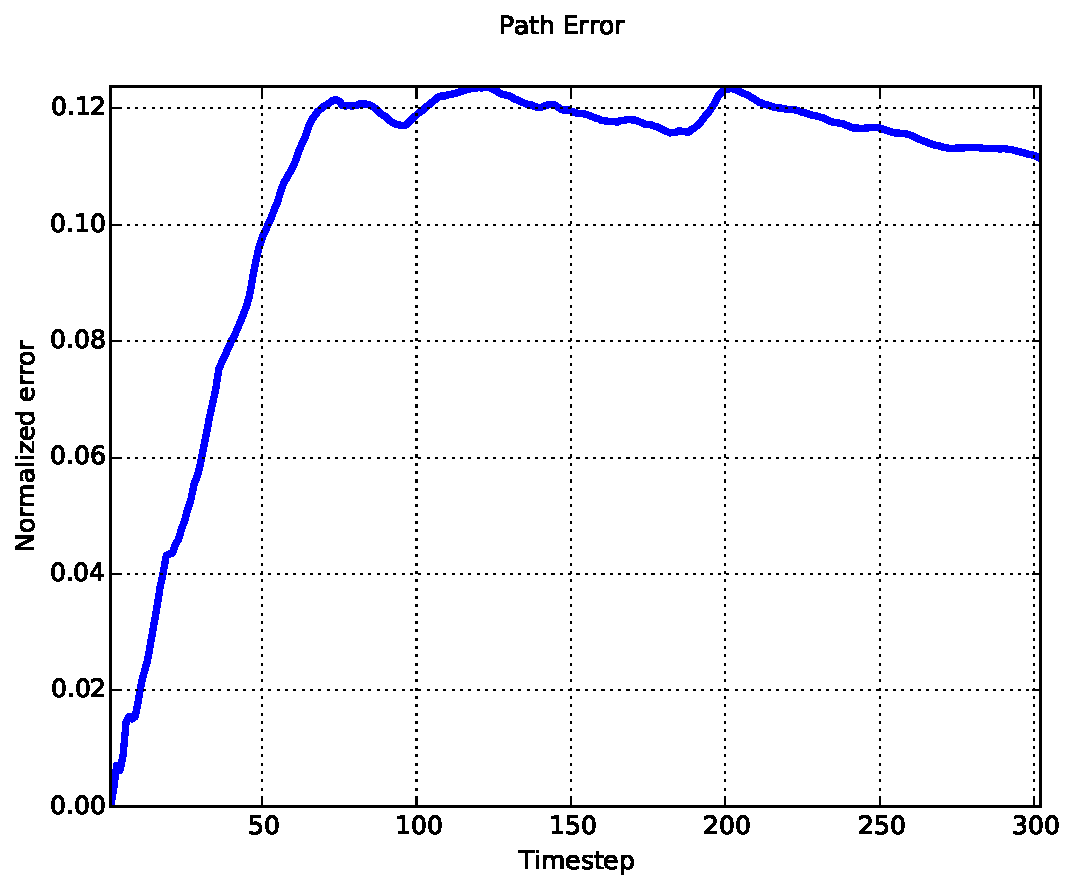
\includegraphics[width=\textwidth]{imagenes/tests/known/res_it_20_nl_40_op_1000_oa_1000_lp_1000_ds_300_kw_1_path.pdf}
\caption{Path normalized error.}
\label{fig:test-ib}
\end{subfigure}
\caption{Results for Test I.}
\label{fig:test-i}
\end{figure}
}
%\clearpage

In the next test all the information parameters of the robot are decreased simultaneously. Is intended to show the effect in the estimation when adding uncertainty to the robot.

\nameref{sec:test-ii}, \nameref{sec:test-iii}, and \nameref{sec:test-iv}, shows the results when $i_{op}=i_{oa}=i_{lp}=100$, $i_{op}=i_{oa}=i_{lp}=10$, and $i_{op}=i_{oa}=i_{lp}=1$ respectively.

%It can be seen that the algorithm can retrieve the path with relative success when the information is 100 and 10, even when the initial guess is very far off. Only when the information is 1, the algorithm breaks.

It can be seen that the estimated path gradually degrades as the the information decrease. Finally when the information is 1, the algorithm breaks.

%\afterpage{
%\clearpage
\subsubsection{Test II}
\label{sec:test-ii}

\begin{table}[htbp!]
    \centering
    \begin{tabular}{|c|c|c|c|c|c|c|}
        \hline
        $n_p$ & $n_l$ & $i_{op}$ & $i_{oa}$ & $i_{lp}$ & $it$ & $k_w$\\
        \hline \hline
        300 & 40 & 100 & 100 & 100 & 20 & 1\\
        \hline 
    \end{tabular}
    \caption{Parameters for Test II.}
    \label{tab:test-ii}
\end{table}

\begin{figure}[htbp!]
    \centering
    \begin{subfigure}[b]{\estWidth\textwidth}
        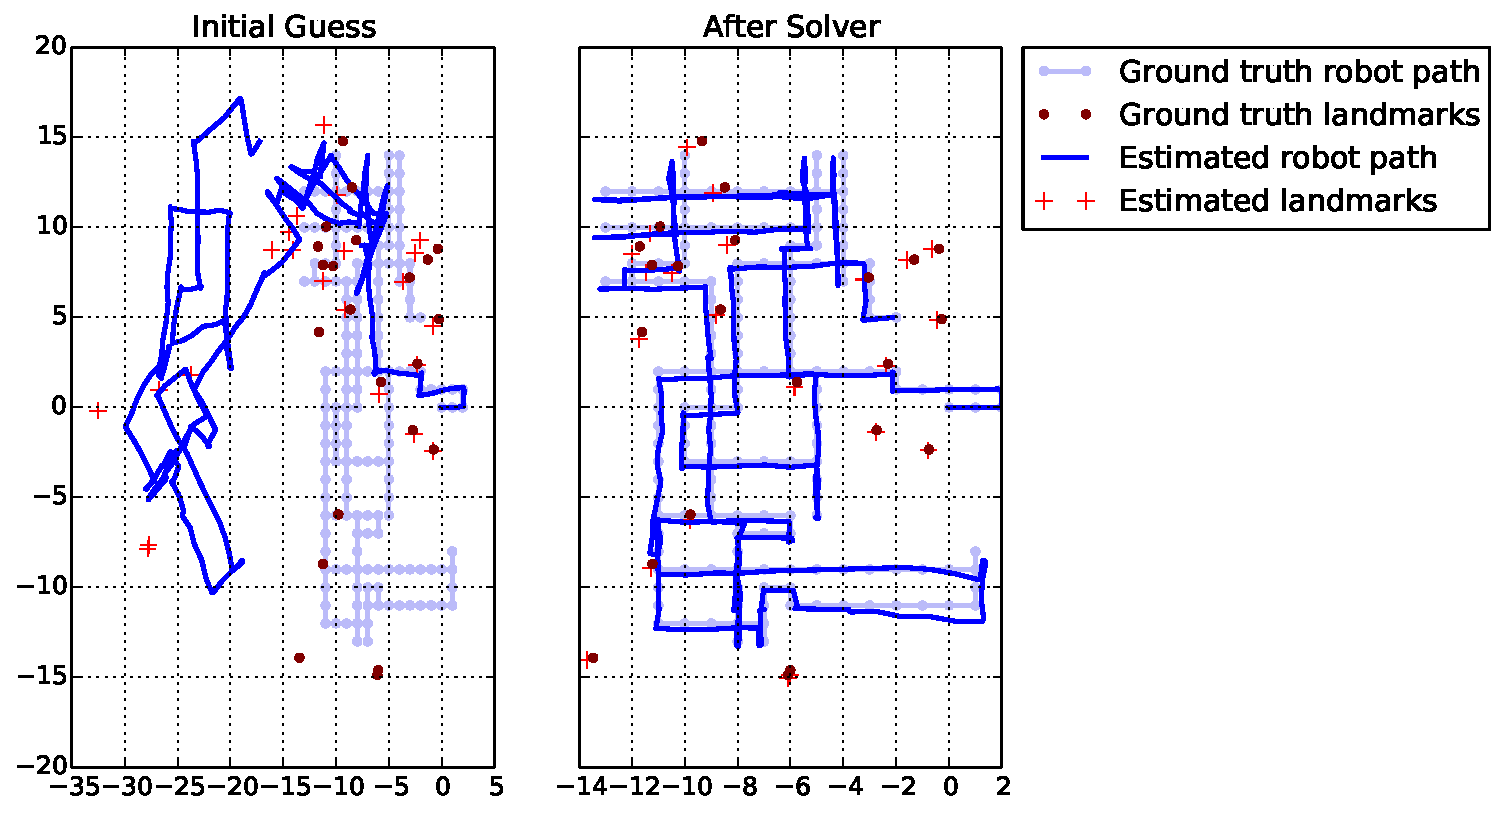
\includegraphics[width=\textwidth]{imagenes/tests/known/res_it_20_nl_40_op_100_oa_100_lp_100_ds_300_kw_1.pdf}
        \caption{Initial guess and solver estimation.}
        \label{fig:test-iia}
    \end{subfigure}\\
    \begin{subfigure}[b]{\errorWidth\textwidth}
        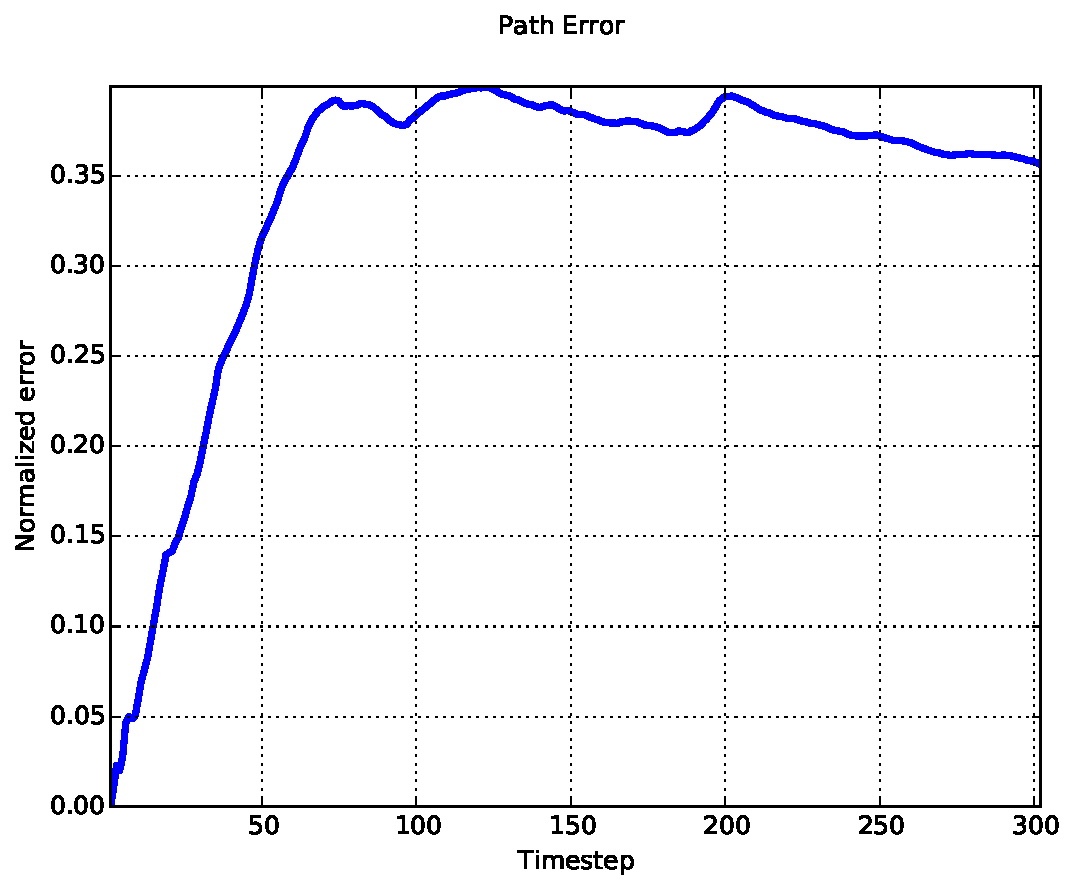
\includegraphics[width=\textwidth]{imagenes/tests/known/res_it_20_nl_40_op_100_oa_100_lp_100_ds_300_kw_1_path.pdf}
        \caption{Path normalized error.}
        \label{fig:test-iib}
    \end{subfigure}
    \caption{Results for Test II.}
    \label{fig:test-ii}
\end{figure}
%}

\afterpage{
\clearpage
\subsubsection{Test III}
\label{sec:test-iii}

\begin{table}[htbp!]
    \centering
    \begin{tabular}{|c|c|c|c|c|c|c|}
        \hline
        $n_p$ & $n_l$ & $i_{op}$ & $i_{oa}$ & $i_{lp}$ & $it$ & $k_w$\\
        \hline \hline
        300 & 40 & 10 & 10 & 10 & 20 & 1\\
        \hline 
    \end{tabular}
    \caption{Parameters for Test III.}
    \label{tab:test-iii}
\end{table}

\begin{figure}[htbp!]
    \centering
    \begin{subfigure}[b]{\estWidth\textwidth}
        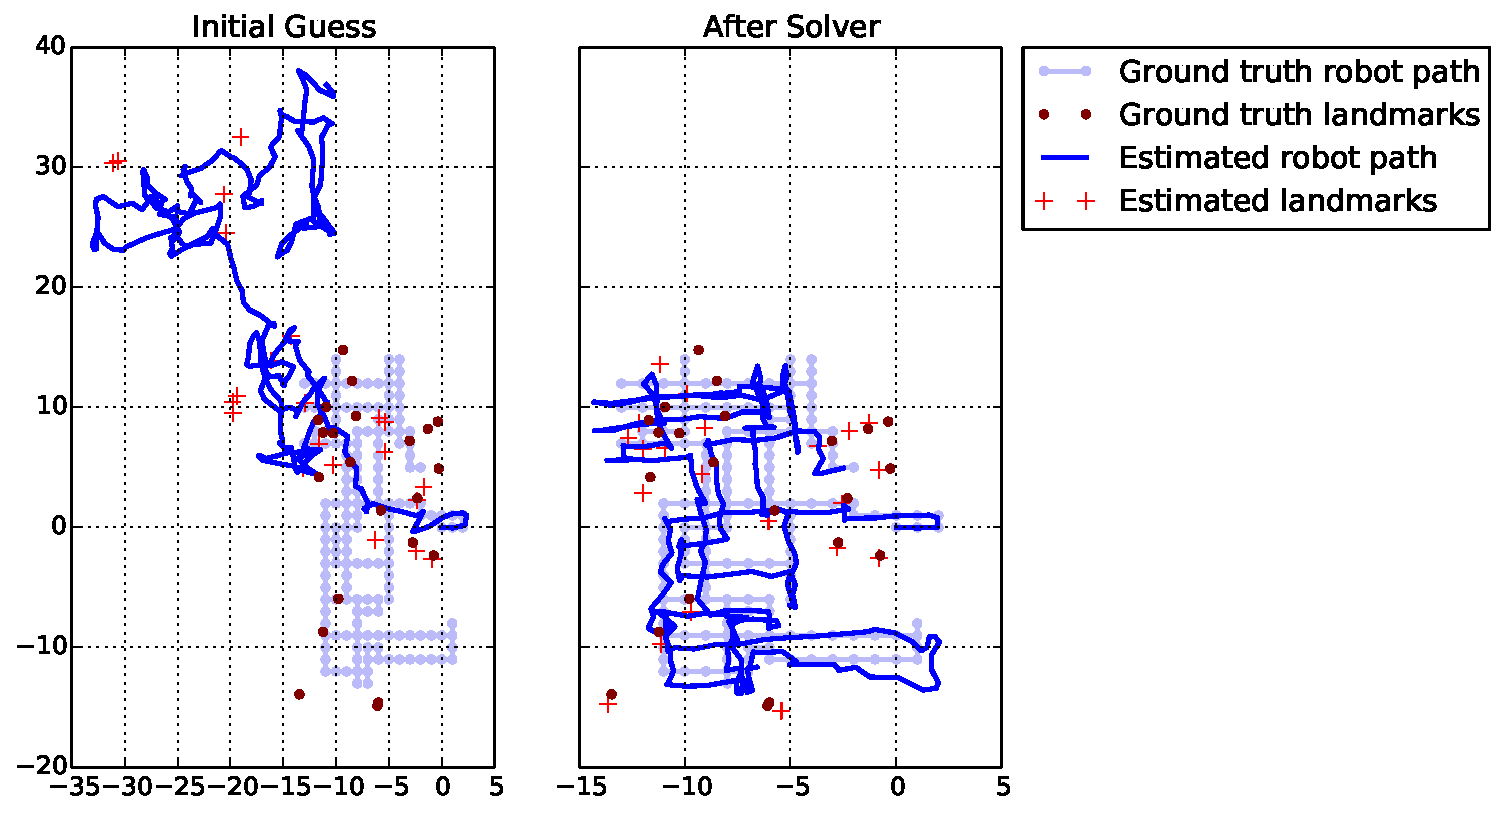
\includegraphics[width=\textwidth]{imagenes/tests/known/res_it_20_nl_40_op_10_oa_10_lp_10_ds_300_kw_1.pdf}
        \caption{Initial guess and solver estimation.}
        \label{fig:test-iiia}
    \end{subfigure}\\
    \begin{subfigure}[b]{\errorWidth\textwidth}
        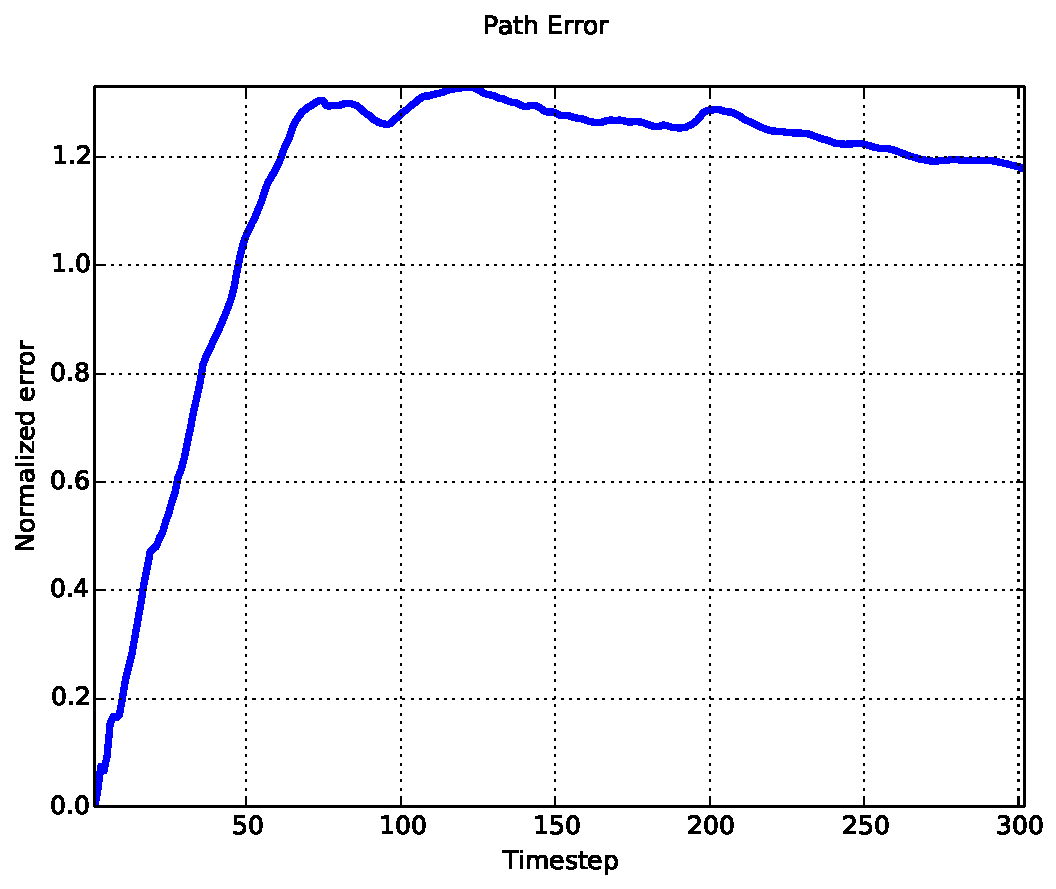
\includegraphics[width=\textwidth]{imagenes/tests/known/res_it_20_nl_40_op_10_oa_10_lp_10_ds_300_kw_1_path.pdf}
        \caption{Path normalized error.}
        \label{fig:test-iiib}
    \end{subfigure}
    \caption{Results for Test III.}
    \label{fig:test-iii}
\end{figure}
}
%\clearpage

\afterpage{
\clearpage
\subsubsection{Test IV}
\label{sec:test-iv}

\begin{table}[htbp!]
    \centering
    \begin{tabular}{|c|c|c|c|c|c|c|}
        \hline
        $n_p$ & $n_l$ & $i_{op}$ & $i_{oa}$ & $i_{lp}$ & $it$ & $k_w$\\
        \hline \hline
        300 & 40 & 1 & 1 & 1 & 20 & 1\\
        \hline 
    \end{tabular}
    \caption{Parameters for Test IV.}
    \label{tab:test-iv}
\end{table}

\begin{figure}[htbp!]
    \centering
    \begin{subfigure}[b]{\estWidth\textwidth}
        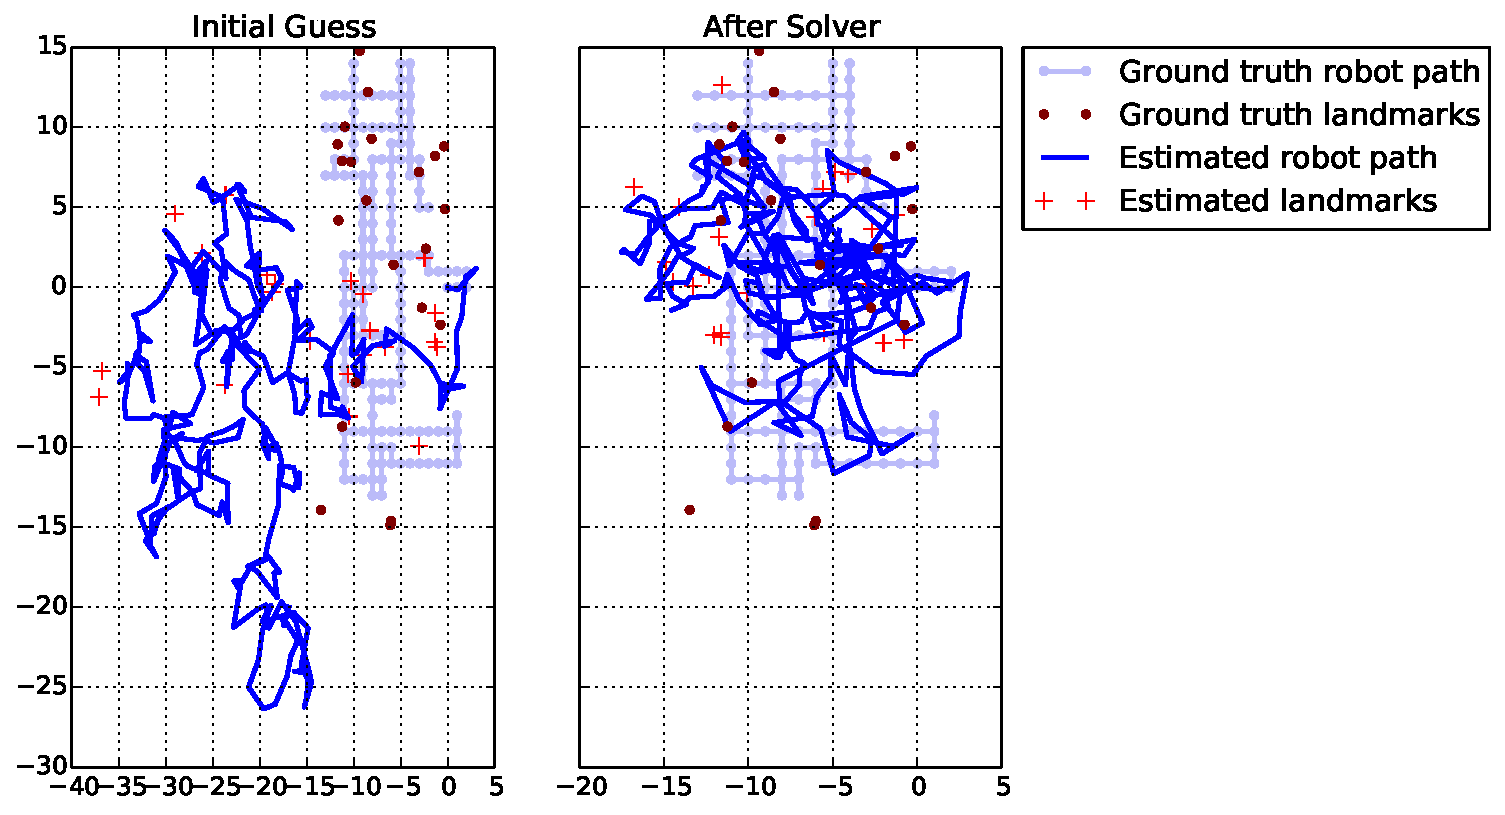
\includegraphics[width=\textwidth]{imagenes/tests/known/res_it_20_nl_40_op_1_oa_1_lp_1_ds_300_kw_1.pdf}
        \caption{Initial guess and solver estimation.}
        \label{fig:test-iva}
    \end{subfigure}\\
    \begin{subfigure}[b]{\errorWidth\textwidth}
        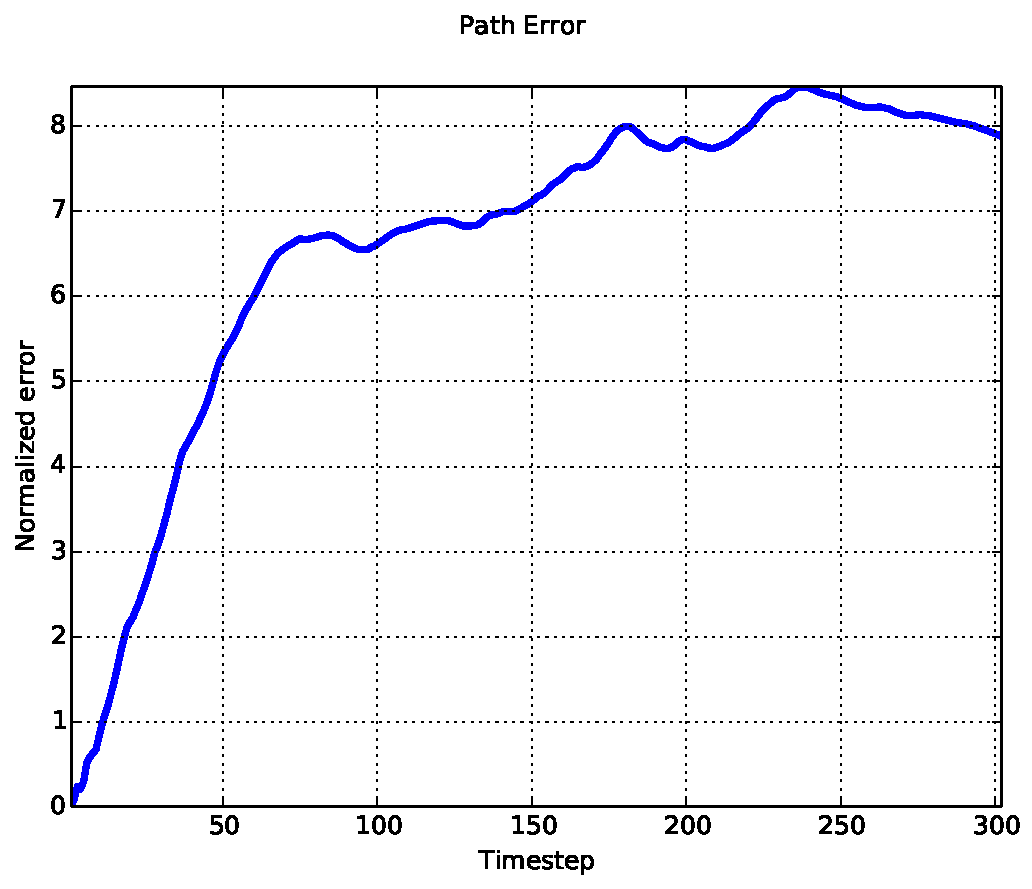
\includegraphics[width=\textwidth]{imagenes/tests/known/res_it_20_nl_40_op_1_oa_1_lp_1_ds_300_kw_1_path.pdf}
        \caption{Path normalized error.}
        \label{fig:test-ivb}
    \end{subfigure}
    \caption{Results for Test IV.}
    \label{fig:test-iv}
\end{figure}
}
%\clearpage

\pagebreak
\nameref{sec:test-v} shows the effect running the algorithm with a low number of iterations. In this case $it=1$. It can be seen that the algorithm was not able to converge properly, in contrast to~\nameref{sec:test-i}.

\afterpage{
\clearpage
\subsubsection{Test V.}
\label{sec:test-v}

\begin{table}[htbp!]
    \centering
    \begin{tabular}{|c|c|c|c|c|c|c|}
        \hline
        $n_p$ & $n_l$ & $i_{op}$ & $i_{oa}$ & $i_{lp}$ & $it$ & $k_w$\\
        \hline \hline
        300 & 40 & 1000 & 1000 & 1000 & 1 & 1\\
        \hline 
    \end{tabular}
    \caption{Parameters for Test V.}
    \label{tab:test-v}
\end{table}

\begin{figure}[htbp!]
    \centering
    \begin{subfigure}[b]{\estWidth\textwidth}
        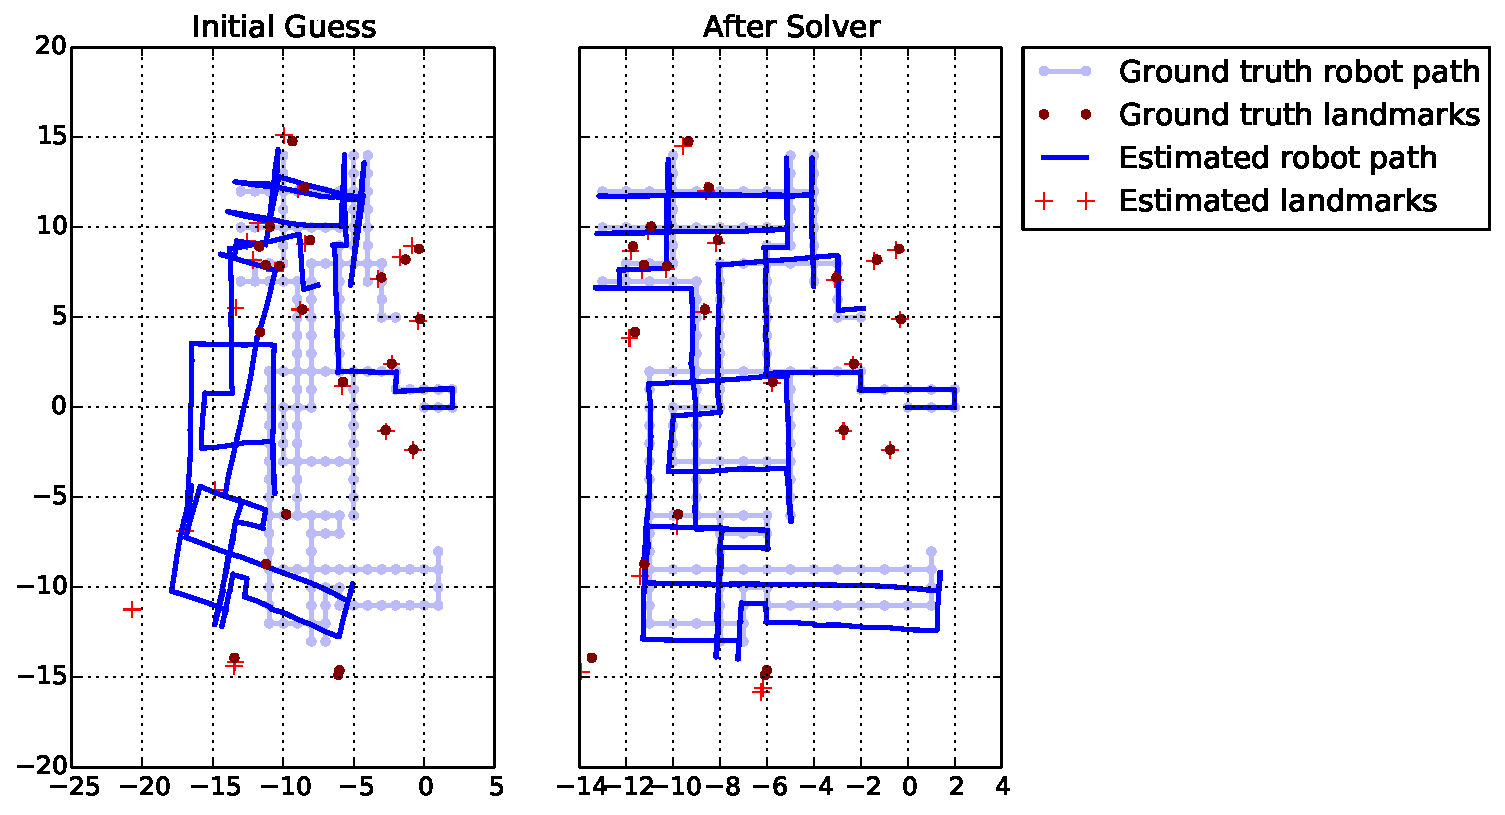
\includegraphics[width=\textwidth]{imagenes/tests/known/res_it_1_nl_40_op_1000_oa_1000_lp_1000_ds_300_kw_1.pdf}
        \caption{Initial guess and solver estimation.}
        \label{fig:test-va}
    \end{subfigure}\\
    \begin{subfigure}[b]{\errorWidth\textwidth}
        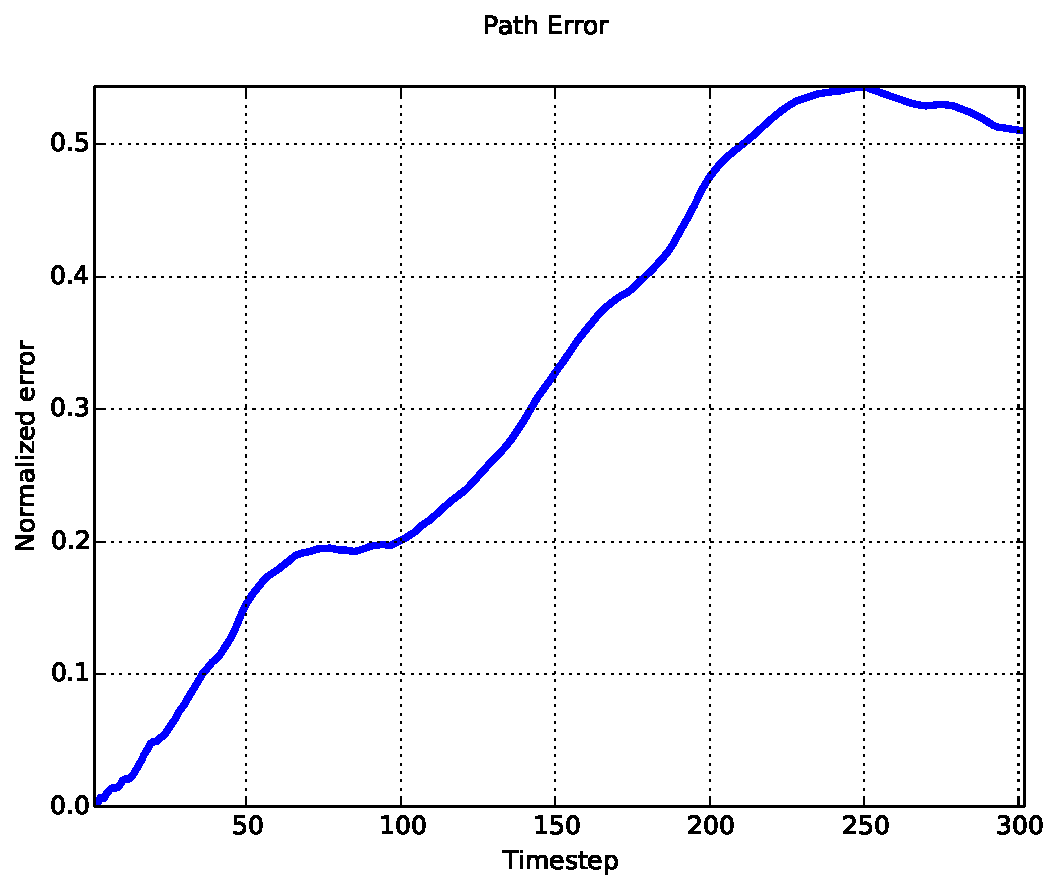
\includegraphics[width=\textwidth]{imagenes/tests/known/res_it_1_nl_40_op_1000_oa_1000_lp_1000_ds_300_kw_1_path.pdf}
        \caption{Path normalized error.}
        \label{fig:test-vb}
    \end{subfigure}
    \caption{Results for Test V.}
    \label{fig:test-v}
\end{figure}
}
%\clearpage

In~\nameref{sec:test-vi} the kernel width was reduced to $k_w=0.1$, meaning the errors are suppressed at a shorter distance. It can be seen that the new width actually improves the results, getting a normalized error for the full path of around 0.08.

\afterpage{
\clearpage
\subsubsection{Test VI.}
\label{sec:test-vi}

\begin{table}[htbp!]
    \centering
    \begin{tabular}{|c|c|c|c|c|c|c|}
        \hline
        $n_p$ & $n_l$ & $i_{op}$ & $i_{oa}$ & $i_{lp}$ & $it$ & $k_w$\\
        \hline \hline
        300 & 40 & 1000 & 1000 & 1000 & 20 & 0.1\\
        \hline 
    \end{tabular}
    \caption{Parameters for Test VI.}
    \label{tab:test-vi}
\end{table}

\begin{figure}[htbp!]
    \centering
    \begin{subfigure}[b]{\estWidth\textwidth}
        \includegraphics[width=\textwidth]{imagenes/tests/known/{res_it_20_nl_40_op_1000_oa_1000_lp_1000_ds_300_kw_0.1}.pdf}
        \caption{Initial guess and solver estimation.}
        \label{fig:test-via}
    \end{subfigure}\\
    \begin{subfigure}[b]{\errorWidth\textwidth}
        \includegraphics[width=\textwidth]{imagenes/tests/known/{res_it_20_nl_40_op_1000_oa_1000_lp_1000_ds_300_kw_0.1_path}.pdf}
        \caption{Path normalized error.}
        \label{fig:test-vib}
    \end{subfigure}
    \caption{Results for Test VI.}
    \label{fig:test-vi}
\end{figure}
}
%\clearpage

In terms of speed the algorithm performs quite fast, taking around $1[s]$ for all the tests.

\pagebreak
\section{Unknown Data Association}
\label{sec:unknown-asso-res}

In this section similar tests are made, but in this case it is assumed unknown data association of the landmarks. The same simulator is used to generate the data, and Algorithm~\ref{alg:final} to compute the estimate.

Along with the parameters used in the known correspondence case, the following new parameters must be set in these tests:

\begin{itemize}
%\setlength\itemsep{1em}
\item $\chi$: likelihood threshold for data association.
\item $dt$: maximum distance for distance test.
\item $io$: inter full optimization frequency.
\item $ps$: Pose skipping.
\end{itemize}

Where $\chi$ and $dt$ are the thresholds used in Algorithm~\ref{alg:incremental-data-association}. $io$ is the number of incremental optimizations between two full optimizations, and $ps$ is the number of poses between optimizations, both form Algorithm~\ref{alg:final}.

\nameref{sec:test-vii} show the results for a successful test with unknown data association. Notice that in the initial guess there are several more landmarks than in the groundtruth. That is because the initial guess consider every single measurement as an independent landmark. However in the result of the solver, the algorithm is able to associate the the measurements with the corresponding landmark, and correct the path of the robot. Nevertheless there are 4 cases that are unable to be associated correctly.

The parameter $dt$ is set to $\infty$ so no distant test is performed. In Table~\ref{tab:test-vii}, variable $t$ correspond to the total time of the algorithm. 

\afterpage{
\clearpage
\subsubsection{Test VII.}
\label{sec:test-vii}

\begin{table}[htbp!]
    \centering
    \begin{tabular}{|c|c|c|c|c|c|c|c|c|c|c|c|}
        \hline
        $n_p$ & $n_l$ & $i_{op}$ & $i_{oa}$ & $i_{lp}$ & $it$ & $k_w$ & $\chi$ & $dt$ & $io$ & $ps$ & $t$\\
        \hline \hline
        400 & 30 & 1000 & 10000 & 1000 & 20 & 1 & 0.1 & $\infty$ & 400 & 10 & $13[s]$\\
        \hline 
    \end{tabular}
    \caption{Parameters for Test VII.}
    \label{tab:test-vii}
\end{table}

\begin{figure}[htbp!]
    \centering
    \begin{subfigure}[b]{\estWidth\textwidth}
        \includegraphics[width=\textwidth]{imagenes/tests/unknown/{res_it_20_xi_0.1_nl_30_op_1000_oa_10000_lp_1000_dsk_1_io_400_ds_400_dt_0_kw_1_ps_10}.pdf}
        \caption{Initial guess and solver estimation.}
        \label{fig:test-viia}
    \end{subfigure}\\
    \begin{subfigure}[b]{\errorWidth\textwidth}
        \includegraphics[width=\textwidth]{imagenes/tests/unknown/{res_it_20_xi_0.1_nl_30_op_1000_oa_10000_lp_1000_dsk_1_io_400_ds_400_dt_0_kw_1_ps_10_path}.pdf}
        \caption{Path normalized error.}
        \label{fig:test-viib}
    \end{subfigure}
    \caption{Results for Test VII.}
    \label{fig:test-vii}
\end{figure}
}
%\clearpage

In the next tests the threshold $\chi$ is modified. In~\nameref{sec:test-viii} the threshold is set to a very low value $\chi=10^{-100}$. It can be seen that the algorithm merges non equivalent landmarks, thus causes estimate divergence.
In~\nameref{sec:test-ix} and \nameref{sec:test-x} $\chi$ is set to 1 and 3 respectively. In these cases the thresholds are so high that the algorithm is unable to associate all the equivalent landmarks. This cause that the estimated path gradually drift.

\afterpage{
\clearpage
\subsubsection{Test VIII.}
\label{sec:test-viii}

\begin{table}[htbp!]
    \centering
    \begin{tabular}{|c|c|c|c|c|c|c|c|c|c|c|c|}
        \hline
        $n_p$ & $n_l$ & $i_{op}$ & $i_{oa}$ & $i_{lp}$ & $it$ & $k_w$ & $\chi$ & $dt$ & $io$ & $ps$ & $t$\\
        \hline \hline
        400 & 30 & 1000 & 10000 & 1000 & 20 & 1 & $10^{-100}$ & $\infty$ & 400 & 10 & $94[s]$\\
        \hline 
    \end{tabular}
    \caption{Parameters for Test VIII.}
    \label{tab:test-viii}
\end{table}

\begin{figure}[htbp!]
    \centering
    \begin{subfigure}[b]{\estWidth\textwidth}
        \includegraphics[width=\textwidth]{imagenes/tests/unknown/{res_it_20_xi_1e-100_nl_30_op_1000_oa_10000_lp_1000_dsk_1_io_400_ds_400_dt_0_kw_1_ps_10}.pdf}
        \caption{Initial guess and solver estimation.}
        \label{fig:test-viiia}
    \end{subfigure}\\
    \begin{subfigure}[b]{\errorWidth\textwidth}
        \includegraphics[width=\textwidth]{imagenes/tests/unknown/{res_it_20_xi_1e-100_nl_30_op_1000_oa_10000_lp_1000_dsk_1_io_400_ds_400_dt_0_kw_1_ps_10_path}.pdf}
        \caption{Path normalized error.}
        \label{fig:test-viiib}
    \end{subfigure}
    \caption{Results for Test VIII.}
    \label{fig:test-viii}
\end{figure}
}
%\clearpage

\afterpage{
\clearpage
\subsubsection{Test IX.}
\label{sec:test-ix}

\begin{table}[htbp!]
    \centering
    \begin{tabular}{|c|c|c|c|c|c|c|c|c|c|c|c|}
        \hline
        $n_p$ & $n_l$ & $i_{op}$ & $i_{oa}$ & $i_{lp}$ & $it$ & $k_w$ & $\chi$ & $dt$ & $io$ & $ps$ & $t$\\
        \hline \hline
        400 & 30 & 1000 & 10000 & 1000 & 20 & 1 & 1 & $\infty$ & 400 & 10 & $10[s]$\\
        \hline 
    \end{tabular}
    \caption{Parameters for Test IX.}
    \label{tab:test-ix}
\end{table}

\begin{figure}[htbp!]
    \centering
    \begin{subfigure}[b]{\estWidth\textwidth}
        \includegraphics[width=\textwidth]{imagenes/tests/unknown/{res_it_20_xi_1_nl_30_op_1000_oa_10000_lp_1000_dsk_1_io_400_ds_400_dt_0_kw_1_ps_10}.pdf}
        \caption{Initial guess and solver estimation.}
        \label{fig:test-ixa}
    \end{subfigure}\\
    \begin{subfigure}[b]{\errorWidth\textwidth}
        \includegraphics[width=\textwidth]{imagenes/tests/unknown/{res_it_20_xi_1_nl_30_op_1000_oa_10000_lp_1000_dsk_1_io_400_ds_400_dt_0_kw_1_ps_10_path}.pdf}
        \caption{Path normalized error.}
        \label{fig:test-ixb}
    \end{subfigure}
    \caption{Results for Test IX.}
    \label{fig:test-ix}
\end{figure}
}
%\clearpage

\afterpage{
\clearpage
\subsubsection{Test X.}
\label{sec:test-x}

\begin{table}[htbp!]
    \centering
    \begin{tabular}{|c|c|c|c|c|c|c|c|c|c|c|c|}
        \hline
        $n_p$ & $n_l$ & $i_{op}$ & $i_{oa}$ & $i_{lp}$ & $it$ & $k_w$ & $\chi$ & $dt$ & $io$ & $ps$ & $t$\\
        \hline \hline
        400 & 30 & 1000 & 10000 & 1000 & 20 & 1 & 3 & $\infty$ & 400 & 10 & $17[s]$\\
        \hline 
    \end{tabular}
    \caption{Parameters for Test X.}
    \label{tab:test-x}
\end{table}

\begin{figure}[htbp!]
    \centering
    \begin{subfigure}[b]{\estWidth\textwidth}
        \includegraphics[width=\textwidth]{imagenes/tests/unknown/{res_it_20_xi_3_nl_30_op_1000_oa_10000_lp_1000_dsk_1_io_400_ds_400_dt_0_kw_1_ps_10}.pdf}
        \caption{Initial guess and solver estimation.}
        \label{fig:test-xa}
    \end{subfigure}\\
    \begin{subfigure}[b]{\errorWidth\textwidth}
        \includegraphics[width=\textwidth]{imagenes/tests/unknown/{res_it_20_xi_3_nl_30_op_1000_oa_10000_lp_1000_dsk_1_io_400_ds_400_dt_0_kw_1_ps_10_path}.pdf}
        \caption{Path normalized error.}
        \label{fig:test-xb}
    \end{subfigure}
    \caption{Results for Test X.}
    \label{fig:test-x}
\end{figure}
}
%\clearpage

In~\nameref{sec:test-xi} $\chi$ gets the value of $\infty$ and $dt=1$, so that in this case the algorithm associates landmarks using the distant test instead of the correspondence test. Every landmark at a distance of 1 unit will be automatically associated. Looking at Figure~\ref{fig:test-xia} it can be seen that now all landmarks are correctly associated. However Figure~\ref{fig:test-xib} shows that the estimation has a greater cumulative error. Also, the distant test is faster than the correspondence test, taking only $5[s]$. Therefore a trade-off exists between using the distant test and the correspondence test as a means to solve unknown association.

\afterpage{
\clearpage
\subsubsection{Test XI.}
\label{sec:test-xi}

\begin{table}[htbp!]
    \centering
    \begin{tabular}{|c|c|c|c|c|c|c|c|c|c|c|c|}
        \hline
        $n_p$ & $n_l$ & $i_{op}$ & $i_{oa}$ & $i_{lp}$ & $it$ & $k_w$ & $\chi$ & $dt$ & $io$ & $ps$ & $t$\\
        \hline \hline
        400 & 30 & 1000 & 10000 & 1000 & 20 & 1 & $\infty$ & 1 & 400 & 10 & $5[s]$\\
        \hline 
    \end{tabular}
    \caption{Parameters for Test XI.}
    \label{tab:test-xi}
\end{table}

\begin{figure}[htbp!]
    \centering
    \begin{subfigure}[b]{\estWidth\textwidth}
        \includegraphics[width=\textwidth]{imagenes/tests/unknown/{res_it_20_xi_0_nl_30_op_1000_oa_10000_lp_1000_dsk_1_io_400_ds_400_dt_1_kw_1_ps_10}.pdf}
        \caption{Initial guess and solver estimation.}
        \label{fig:test-xia}
    \end{subfigure}\\
    \begin{subfigure}[b]{\errorWidth\textwidth}
        \includegraphics[width=\textwidth]{imagenes/tests/unknown/{res_it_20_xi_0_nl_30_op_1000_oa_10000_lp_1000_dsk_1_io_400_ds_400_dt_1_kw_1_ps_10_path}.pdf}
        \caption{Path normalized error.}
        \label{fig:test-xib}
    \end{subfigure}
    \caption{Results for Test XI.}
    \label{fig:test-xi}
\end{figure}
}
%\clearpage

In~\nameref{sec:test-xii} the pose skip parameter is increase to $ps=100$. the idea is to do as least optimization as possible to increase the algorithm speed. It can be seen however that, due to the lack of optimization, the algorithm is unable to correct the path and to associate the landmarks. This errors also cause that the algorithm actually takes longer than in~\nameref{sec:test-vii}. 

\afterpage{
\clearpage
\subsubsection{Test XII.}
\label{sec:test-xii}

\begin{table}[htbp!]
    \centering
    \begin{tabular}{|c|c|c|c|c|c|c|c|c|c|c|c|}
        \hline
        $n_p$ & $n_l$ & $i_{op}$ & $i_{oa}$ & $i_{lp}$ & $it$ & $k_w$ & $\chi$ & $dt$ & $io$ & $ps$ & $t$\\
        \hline \hline
        400 & 30 & 1000 & 10000 & 1000 & 20 & 1 & 0.1 & $\infty$ & 400 & 100 & $21[s]$\\
        \hline 
    \end{tabular}
    \caption{Parameters for Test XII.}
    \label{tab:test-xii}
\end{table}

\begin{figure}[htbp!]
    \centering
    \begin{subfigure}[b]{\estWidth\textwidth}
        \includegraphics[width=\textwidth]{imagenes/tests/unknown/{res_it_20_xi_0.1_nl_30_op_1000_oa_10000_lp_1000_dsk_1_io_400_ds_400_dt_0_kw_1_ps_100}.pdf}
        \caption{Initial guess and solver estimation.}
        \label{fig:test-xiia}
    \end{subfigure}\\
    \begin{subfigure}[b]{\errorWidth\textwidth}
        \includegraphics[width=\textwidth]{imagenes/tests/unknown/{res_it_20_xi_0.1_nl_30_op_1000_oa_10000_lp_1000_dsk_1_io_400_ds_400_dt_0_kw_1_ps_100_path}.pdf}
        \caption{Path normalized error.}
        \label{fig:test-xiib}
    \end{subfigure}
    \caption{Results for Test XII.}
    \label{fig:test-xii}
\end{figure}
}
%\clearpage
 
\pagebreak
\section{Real Data}
\label{sec:real-data-res} 

In this section the correctness of the algorithm is proven for more realistic data. The size of the data is much larger than the previous cases, the number of poses in a path are in the order of thousands and ten thousands. Unfortunately the amount of data is so large, that it becomes infeasible to apply the correspondence test, because it so computationally expensive it takes several hours to run the algorithm. For this reason, only the distant test is used. Moreover, the data presents undesired properties like non-Gaussian noise and false alarms, nevertheless it'll be shown that it's still possible to apply the algorithm and get good results.

\subsection{Husky a200 Robot}

The first of these test is a Husky a200 Robot simulated in Gazebo. Since this test is still a simulation the groundtruth and the path error can still be retrieved. However, since Gazebo is a more realistic simulation, the nonlinear models of the robot, miss in the detections and false alarms are also simulated. 

The parameters of the algorithm are presented it Table~\ref{tab:test-xiii}. In this case the information parameters $i_{op}$, $i_{oa}$, and $i_{lp}$ are the assumed uncertainty that better fit the robot model. Since no knowledge was acquired about the robot, these parameters were chosen by trial and error. 

The result are shown in Figure~\ref{fig:test-xiii}. It can be seen that the algorithm can correctly predict the robot path. Most of the landmarks are also found, but there a lot of false positives, possibly generated by sensor malfunctions, spurious measurements, or moving objects. A possible way to get rid of these false alarms is to apply a policy of elimination of landmarks if they are not measured a certain number of times. Nevertheless, the false alarms do not affect greatly the results of the estimation.

\afterpage{
\clearpage
\subsubsection{Test XIII.}
\label{sec:test-xiii}

\begin{table}[htbp!]
    \centering
    \begin{tabular}{|c|c|c|c|c|c|c|c|c|c|c|c|}
        \hline
        $n_p$ & $n_l$ & $i_{op}$ & $i_{oa}$ & $i_{lp}$ & $it$ & $k_w$ & $\chi$ & $dt$ & $io$ & $ps$ & $t$\\
        \hline \hline
        4700 & 18 & 10000 & 10000 & 1000 & 10 & 1 & $\infty$ & 0.5 & 500 & 10 & $3[min]$\\
        \hline 
    \end{tabular}
    \caption{Parameters for Test XIII.}
    \label{tab:test-xiii}
\end{table}

\begin{figure}[htbp!]
    \centering
    \begin{subfigure}[b]{\estWidth\textwidth}
        \includegraphics[width=\textwidth]{imagenes/tests/real/{res_ROS_2015-12-11 19:29:05_it_10_xi_0_op_10000_oa_10000_lp_1000_dsk_1_io_500_ds_100000_dt_0.5_kw_1_ps_10}.pdf}
        \caption{Initial guess and solver estimation.}
        \label{fig:test-xiiia}
    \end{subfigure}\\
    \begin{subfigure}[b]{\errorWidth\textwidth}
        \includegraphics[width=\textwidth]{imagenes/tests/real/{res_ROS_2015-12-11 19:29:05_it_10_xi_0_op_10000_oa_10000_lp_1000_dsk_1_io_500_ds_100000_dt_0.5_kw_1_ps_10_path}.pdf}
        \caption{Path normalized error.}
        \label{fig:test-xiiib}
    \end{subfigure}
    \caption{Results for Test XIII.}
    \label{fig:test-xiii}
\end{figure}
}
%\clearpage

\subsection{Parque O'Higgins}

This dataset corresponds to data taken in Parque O'Higgins by a robot from Universidad de Chile. Since this is real data there is no groundtruth with which compare the results. However, the robot was controlled so that it return to the starting position at the end of the path, so it is possible to check the correctness of the algorithm by looking at the robot's final position. Also, since there is no groudtruth there no way to known the correct amount to landmarks in the map.

The results are shown in~\nameref{sec:test-xiv}, along with the parameters used in the test. It can be seen that in the initial guess the robot doesn't return to the starting position (0,0), however it does when the algorithm is applied, thus proving the correctness of the estimate. Due to the large size of the data the algorithm took 4 hours to finish.

\afterpage{
\clearpage
\subsubsection{Test XIV.}
\label{sec:test-xiv}

\begin{table}[htbp!]
    \centering
    \begin{tabular}{|c|c|c|c|c|c|c|c|c|c|c|c|}
        \hline
        $n_p$ & $n_l$ & $i_{op}$ & $i_{oa}$ & $i_{lp}$ & $it$ & $k_w$ & $\chi$ & $dt$ & $io$ & $ps$ & $t$\\
        \hline \hline
        8130 & - & 100000 & 100000 & 100 & 10 & 1 & $\infty$ & 3 & 500 & 10 & $4[hrs]$\\
        \hline 
    \end{tabular}
    \caption{Parameters for Test XIV.}
    \label{tab:test-xiv}
\end{table}

\begin{figure}[htbp!]
    \centering
    \includegraphics[width=\estWidth\textwidth]{imagenes/tests/real/{res_ohiggins_2015-12-11 23:49:28_it_10_xi_0_op_100000_oa_100000_lp_100_dsk_1_io_500_ds_100000_dt_3_kw_1_ps_10}.pdf}
    \caption{Results for Test XIV.}
    \label{fig:test-xiv}
\end{figure}
}
%\clearpage

%\pagebreak
\subsection{Victoria Park}

The Victoria Park\footnote{Avaliable in \url{http://www.mrpt.org/Dataset_The_Victoria_Park}} is as commonly used datatest to test algorithms related to localization, mapping and SLAM. No real groundtruth of the map exists, however in this case the results can be compared with ones obtained by similar algorithms. 

\nameref{sec:test-xv} show the results of the algorithm in the Victoria Park dataset. In Figure~\ref{fig:victoria-graphslam-isam} the results are compared with the iSAM algorithm~\cite{isam} for the same dataset. It can be appreciated the resemblance between the two results. The main difference is the number of landmarks, since this implementation of GraphSLAM does not have a way to eliminate false alarms, they will stay forever in the map. The main disadvantage of the GraphSLAM algorithm is the computation time, due to the size of the dataset, it took 10 hours to finish.

\afterpage{
\clearpage
\subsubsection{Test XV.}
\label{sec:test-xv}

\begin{table}[htbp!]
    \centering
    \begin{tabular}{|c|c|c|c|c|c|c|c|c|c|c|c|}
        \hline
        $n_p$ & $n_l$ & $i_{op}$ & $i_{oa}$ & $i_{lp}$ & $it$ & $k_w$ & $\chi$ & $dt$ & $io$ & $ps$ & $t$\\
        \hline \hline
        61763 & - & 8000 & 100000 & 5 & 15 & 1 & $\infty$ & 5 & 500 & 10 & $10[hrs]$\\
        \hline 
    \end{tabular}
    \caption{Parameters for Test XV.}
    \label{tab:test-xv}
\end{table}

\begin{figure}[htbp!]
    \centering
    \includegraphics[width=\estWidth\textwidth]{imagenes/tests/real/{res_victoria_2015-12-14 01:28:19_it_15_xi_0_op_8000_oa_100000_lp_5_dsk_1_io_500_ds_100000_dt_5_kw_1_ps_10}.pdf}
    \caption{Results for Test XV.}
    \label{fig:test-xv}
\end{figure}
}

\afterpage{
\clearpage
\begin{figure}[htbp!]
    \centering
    \begin{subfigure}[b]{0.6\textwidth}
        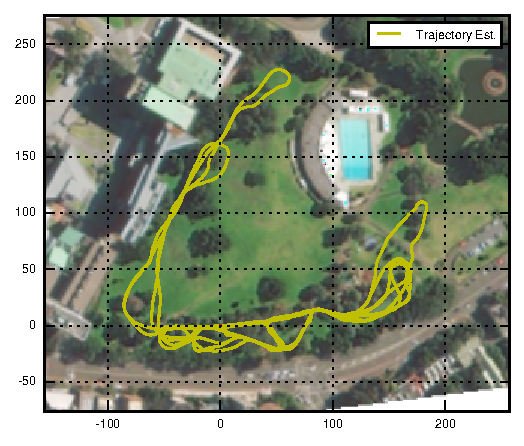
\includegraphics[width=\textwidth]{imagenes/estimate.pdf}
        \caption{Results GraphSLAM in the Victoria Park dataset (trajectory only).}
        \label{fig:victoria-graphslam}
    \end{subfigure}
    \\
    \centering
    \begin{subfigure}[b]{0.5\textwidth}
    \hspace{-2cm}
    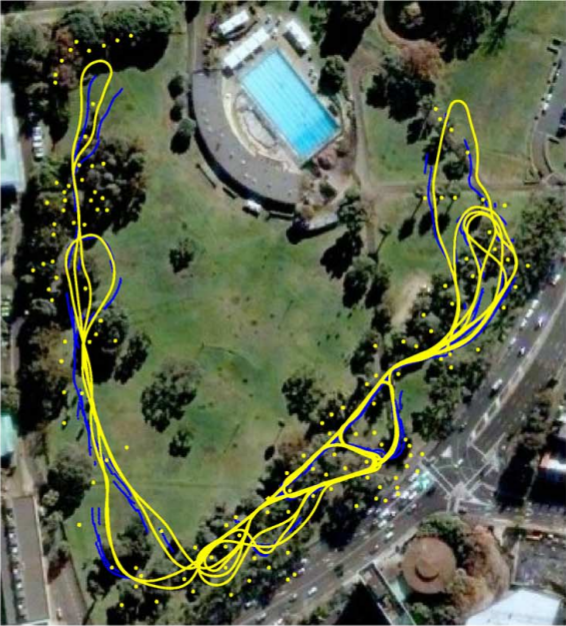
\includegraphics[width=\textwidth, angle=-36]{imagenes/victoria-isam.png}
    \caption{Results iSAM in the Victoria Park dataset~\cite{isam}.}
    \label{fig:victoria-isam}
    \end{subfigure}
    \caption{Comparison of results between GraphSLAM and iSAM.}
    \label{fig:victoria-graphslam-isam}
\end{figure}
}

\newpage
\chapter{Conclusions}
\label{chap:conclusion}

In the present work, the GraphSLAM algorithm was implemented for solving the SLAM problem in the 2D scenario. The g$^2$o framework provided to be a good tool for least squares nonlinear optimization, and it includes kernels methods for robust estimation. The algorithm makes some assumptions about the robot models, in particular, it assumes zero-mean white Gaussian noise and the Markov condition. However, GraphSLAM proved to be robust to outliers and non-Gaussian noise.

The GraphSLAM implementation is able to deal with known and unknown data association of the landmarks. The known data association case is a simple application of the g$^2$o framework with the right parameters. The unknown data association is a more complicated case since there is no a straightforward way to deal with it. A method of maximum likelihood was developed using the uncertainty information that can be retrieved from g$^2$o to create a correspondence test. Then this test was applied iteratively to give a solution to the unknown correspondence. To speed up the algorithm several strategies were implemented: incremental optimization, pose skipping and distant test, all were able to decrease significantly the computational time.

The GraphSLAM algorithm was also designed to be fine-tuned, with several parameters for the user to set. these parameters include the information in the robot model, the number of iterations of the optimization algorithm, the kernel width, the number of full optimizations, and the threshold of the correspondence and distant tests. 

The algorithm was tested with simulated and real data, for known and unknown data association. The algorithm performed satisfactorily, being able to correct the path in all the tested cases, and achieved a low error when the ground truth was available. It was even able to work correctly with real data, where several assumption about the robot model and the data no longer hold. The implementation was also able to get results comparables with popular algorithms like iSAM.

%The correctness of the results was confirmed checking imposed condition on the data, and comparing with similar implementations. 

A parameter analysis was made for several test scenarios, from which is concluded that a thorough choice of some parameters must be made for the algorithm to work correctly, while others parameters affect the convergence speed. The biggest drawbacks of the algorithm are the computation time, that can take in the order of hours for large datasets, and the trial-and-error tuning of the parameters that has to be made if no prior information of the robot model is known. 

As future work it is suggested to improve the algorithm speed, for example, by incrementally constructing the graph to optimize in g$^2$o. Another unsolved issue in this work is the management of false positives. It is suggested to implement a policy to discard landmarks that are observed only a limited number of times, especially when future observations doesn't find landmarks where they should. The algorithm could also be extended to work in the 3 dimensional case. This extension shouldn't be difficult since g$^2$o already support nodes and edges of three dimensions. 


\bibliographystyle{plain}
\bibliography{bibliografia}

% \input{anexo_apendices.tex} % opcionales

\end{document}
